\documentclass[11pt,a4paper]{article}

% ── Packages ──────────────────────────────────────────────────────────
\usepackage[utf8]{inputenc}
\usepackage[T1]{fontenc}
\usepackage{amsmath,amssymb,amsthm}
\usepackage{mathtools}
\usepackage{bm}
\usepackage{physics}
\usepackage{graphicx}
\usepackage{float}
\usepackage{booktabs}
\usepackage{array}
\usepackage{geometry}
\usepackage{hyperref}
\usepackage{cleveref}
\usepackage{tikz}
\usetikzlibrary{angles,quotes,calc,arrows.meta,decorations.markings,patterns}
\usepackage{caption}
\usepackage{subcaption}
\usepackage{enumitem}
\usepackage{xcolor}
\usepackage{tcolorbox}
\usepackage{fancyhdr}

\geometry{margin=2.5cm}
\hypersetup{colorlinks=true, linkcolor=blue!70!black, citecolor=green!50!black, urlcolor=blue!60!black}

% ── Custom commands ───────────────────────────────────────────────────
\newcommand{\vc}[1]{\bm{#1}}
\newcommand{\mat}[1]{\bm{#1}}
\newcommand{\dt}[1]{\dot{#1}}
\newcommand{\ddt}[1]{\ddot{#1}}
\newcommand{\pder}[2]{\frac{\partial #1}{\partial #2}}
\newcommand{\thetaone}{\theta_1}
\newcommand{\thetatwo}{\theta_2}
\newcommand{\thetathree}{\theta_3}

% ── Fix hyperref bookmark conflicts with custom commands ──────────────
\pdfstringdefDisableCommands{%
  \def\vc#1{#1}%
  \def\mat#1{#1}%
  \def\dt#1{#1}%
  \def\ddt#1{#1}%
  \def\bm#1{#1}%
}

\newtcolorbox{keybox}[1][]{colback=blue!5!white, colframe=blue!50!black, title=#1, fonttitle=\bfseries}
\newtcolorbox{resultbox}[1][]{colback=red!5!white, colframe=red!50!black, title=#1, fonttitle=\bfseries}

% ── Header ────────────────────────────────────────────────────────────
\pagestyle{fancy}
\fancyhead[L]{\small H-Walker Biomechanical Model}
\fancyhead[R]{\small \thepage}
\fancyfoot{}

\title{
    \vspace{-1cm}
    {\LARGE \textbf{Three-Link Planar Biomechanical Model}} \\[0.3cm]
    {\Large \textbf{for Human Gait Analysis}} \\[0.5cm]
    {\large Complete Nonlinear Euler--Lagrange Derivation} \\[0.3cm]
    {\normalsize H-Walker Cable-Driven Walking Rehabilitation Robot}
}
\author{H-Walker Research Team}
\date{April 2026}

\begin{document}
\maketitle
\tableofcontents
\newpage

% ======================================================================
% SECTION 1: INTRODUCTION
% ======================================================================
\section{Introduction}

This document presents a complete derivation of the nonlinear equations of
motion for a three-link planar biomechanical model of the human lower limb
during gait. The model represents the \textbf{thigh}, \textbf{shank}, and
\textbf{foot} as three rigid links connected by revolute joints at the
\textbf{hip}, \textbf{knee}, and \textbf{ankle}.

\subsection{Purpose}
\begin{itemize}
    \item Provide a mathematically rigorous model for the H-Walker cable-driven
          rehabilitation robot.
    \item Enable model-based control: impedance control, ILC (Iterative Learning
          Control), and MPC (Model Predictive Control).
    \item Compute inverse dynamics torques from measured joint trajectories.
    \item Map cable tension forces to equivalent joint torques.
\end{itemize}

\subsection{Assumptions}
\begin{enumerate}
    \item \textbf{Planar (2D) sagittal plane model}: All motion occurs in the sagittal plane.
          Abduction/adduction and internal/external rotation are neglected.
    \item \textbf{Rigid body segments}: Each segment (thigh, shank, foot) is a rigid body
          with constant mass, length, and inertia.
    \item \textbf{Frictionless joints}: Joint friction is neglected
          (can be added as viscous damping
          $\tau_{\text{friction},i} = -b_i \dt{\theta}_i$).
    \item \textbf{Fixed hip}: During swing phase analysis, the hip is treated as a
          fixed pivot point. During stance, hip motion can be prescribed.
    \item \textbf{Point masses at CoM}: The mass of each segment is concentrated at
          its center of mass, with a rotational inertia about the CoM.
\end{enumerate}

\subsection{Notation Summary}

\begin{table}[H]
\centering
\caption{Symbol definitions used throughout this document.}
\label{tab:notation}
\begin{tabular}{@{}cll@{}}
\toprule
\textbf{Symbol} & \textbf{Description} & \textbf{Unit} \\
\midrule
$m_i$ & Mass of segment $i$ & kg \\
$l_i$ & Length of segment $i$ & m \\
$l_{c_i}$ & Distance from proximal joint to CoM of segment $i$ & m \\
$I_i$ & Moment of inertia of segment $i$ about its CoM & kg$\cdot$m$^2$ \\
$\theta_i$ & Absolute angle of segment $i$ from downward vertical & rad \\
$\dt{\theta}_i$ & Angular velocity of segment $i$ & rad/s \\
$\ddt{\theta}_i$ & Angular acceleration of segment $i$ & rad/s$^2$ \\
$\tau_i$ & Generalized torque at joint $i$ & N$\cdot$m \\
$g$ & Gravitational acceleration ($9.81$) & m/s$^2$ \\
\midrule
$s_i$ & $\sin(\theta_i)$ & -- \\
$c_i$ & $\cos(\theta_i)$ & -- \\
$s_{ij}$ & $\sin(\theta_i - \theta_j)$ & -- \\
$c_{ij}$ & $\cos(\theta_i - \theta_j)$ & -- \\
\midrule
$i=1$ & Thigh (hip $\to$ knee) & -- \\
$i=2$ & Shank (knee $\to$ ankle) & -- \\
$i=3$ & Foot (ankle $\to$ toe) & -- \\
\bottomrule
\end{tabular}
\end{table}

% ======================================================================
% SECTION 2: COORDINATE SYSTEM
% ======================================================================
\section{Coordinate System and Generalized Coordinates}

\subsection{Reference Frame}

We adopt a right-handed Cartesian coordinate system with:
\begin{itemize}
    \item Origin at the \textbf{hip joint}
    \item $x$-axis pointing \textbf{forward} (direction of walking)
    \item $y$-axis pointing \textbf{upward}
\end{itemize}

\subsection{Generalized Coordinates}

The system has \textbf{3 degrees of freedom}. We use \textit{absolute angles}
measured from the downward vertical:

\begin{keybox}[Generalized Coordinates]
\begin{equation}
    \vc{q} = \begin{bmatrix} \theta_1 \\ \theta_2 \\ \theta_3 \end{bmatrix}
    \label{eq:gen_coords}
\end{equation}
where each $\theta_i$ is measured from the \textbf{negative $y$-axis}
(downward vertical), positive in the \textbf{counterclockwise} direction
(forward flexion).
\begin{itemize}
    \item $\theta_i = 0$: Segment $i$ hangs straight down (equilibrium)
    \item $\theta_i > 0$: Segment rotated forward (flexion)
    \item $\theta_i < 0$: Segment rotated backward (extension)
\end{itemize}
\end{keybox}

\subsection{Relationship to Clinical Joint Angles}

Clinical gait analysis uses \textit{relative} (joint) angles. The conversion is:

\begin{align}
    \phi_{\text{hip}} &= \theta_1 \label{eq:hip_rel} \\
    \phi_{\text{knee}} &= \theta_1 - \theta_2 \label{eq:knee_rel} \\
    \phi_{\text{ankle}} &= \theta_2 - \theta_3 + \frac{\pi}{2} \label{eq:ankle_rel}
\end{align}

Inverse:
\begin{align}
    \theta_1 &= \phi_{\text{hip}} \\
    \theta_2 &= \phi_{\text{hip}} - \phi_{\text{knee}} \\
    \theta_3 &= \phi_{\text{hip}} - \phi_{\text{knee}} - \phi_{\text{ankle}} + \frac{\pi}{2}
\end{align}

\subsection{Model Diagram}

\begin{figure}[H]
\centering
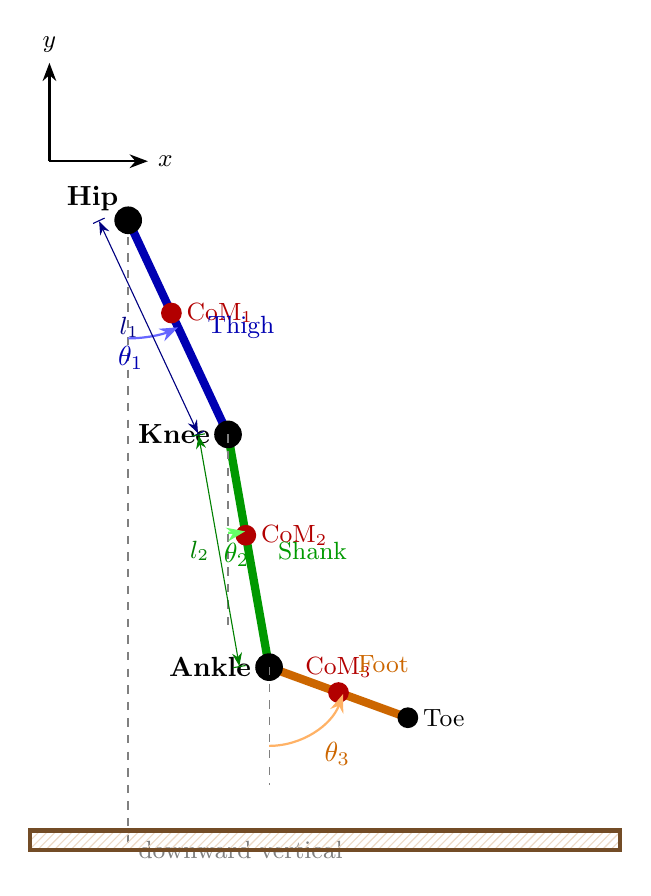
\begin{tikzpicture}[scale=2.5, >=Stealth]
    % Vertical reference
    \draw[dashed, gray, thick] (0,0) -- (0,-3.2) node[right, gray]{\small downward vertical};

    % Thigh
    \coordinate (hip) at (0,0);
    \coordinate (knee) at ({1.2*sin(25)},{-1.2*cos(25)});
    \draw[blue!70!black, line width=3pt] (hip) -- (knee);

    % Shank
    \coordinate (ankle) at ($(knee) + ({1.2*sin(10)},{-1.2*cos(10)})$);
    \draw[green!60!black, line width=3pt] (knee) -- (ankle);

    % Foot
    \coordinate (toe) at ($(ankle) + ({0.75*sin(70)},{-0.75*cos(70)})$);
    \draw[orange!80!black, line width=3pt] (ankle) -- (toe);

    % Ground
    \draw[brown!60!black, line width=1.5pt, pattern=north east lines, pattern color=brown!30]
        (-0.5, -3.1) rectangle (2.5, -3.2);

    % Joint markers
    \fill[black] (hip) circle (2pt) node[above left]{\textbf{Hip}};
    \fill[black] (knee) circle (2pt) node[left=3pt]{\textbf{Knee}};
    \fill[black] (ankle) circle (2pt) node[left=3pt]{\textbf{Ankle}};
    \fill[black] (toe) circle (1.5pt) node[right=2pt]{\small Toe};

    % CoM markers
    \coordinate (com1) at ($(hip)!0.433!(knee)$);
    \coordinate (com2) at ($(knee)!0.433!(ankle)$);
    \coordinate (com3) at ($(ankle)!0.5!(toe)$);
    \fill[red!70!black] (com1) circle (1.5pt) node[right=2pt]{\small $\text{CoM}_1$};
    \fill[red!70!black] (com2) circle (1.5pt) node[right=2pt]{\small $\text{CoM}_2$};
    \fill[red!70!black] (com3) circle (1.5pt) node[above=2pt]{\small $\text{CoM}_3$};

    % Angle arcs
    \draw[blue!60, thick, ->] (0,-0.6) arc[start angle=270, end angle=295, radius=0.6]
        node[midway, below left]{\color{blue!70!black}$\theta_1$};

    % Vertical at knee
    \draw[dashed, gray, thin] (knee) -- ($(knee) + (0,-1.0)$);
    \draw[green!60, thick, ->] ($(knee) + (0,-0.5)$) arc[start angle=270, end angle=280, radius=0.5]
        node[midway, below]{\color{green!60!black}$\theta_2$};

    % Vertical at ankle
    \draw[dashed, gray, thin] (ankle) -- ($(ankle) + (0,-0.6)$);
    \draw[orange!60, thick, ->] ($(ankle) + (0,-0.4)$) arc[start angle=270, end angle=340, radius=0.4]
        node[midway, below right]{\color{orange!80!black}$\theta_3$};

    % Length labels
    \draw[|<->|, blue!50!black] ($(hip) + (-0.15,0)$) -- ($(knee) + (-0.15,0)$)
        node[midway, left]{\small $l_1$};
    \draw[|<->|, green!50!black] ($(knee) + (-0.15,0)$) -- ($(ankle) + (-0.15,0)$)
        node[midway, left]{\small $l_2$};

    % Coordinate axes
    \draw[->, thick, black] (-0.4, 0.3) -- (0.1, 0.3) node[right]{\small $x$};
    \draw[->, thick, black] (-0.4, 0.3) -- (-0.4, 0.8) node[above]{\small $y$};

    % Labels
    \node[blue!70!black, right] at ($(hip)!0.5!(knee) + (0.1,0)$) {\small Thigh};
    \node[green!60!black, right] at ($(knee)!0.5!(ankle) + (0.1,0)$) {\small Shank};
    \node[orange!80!black, above right] at ($(ankle)!0.5!(toe) + (0.05,0.05)$) {\small Foot};
\end{tikzpicture}
\caption{Three-link planar model of the lower limb. Angles $\theta_1$, $\theta_2$,
$\theta_3$ are absolute angles measured from the downward vertical (positive = CCW).
Red dots indicate centers of mass.}
\label{fig:three_link_diagram}
\end{figure}


% ======================================================================
% SECTION 3: POSITION KINEMATICS
% ======================================================================
\section{Position Kinematics}

With the hip at the origin, we derive the position of every joint and
center of mass as functions of the generalized coordinates $\vc{q}$.

\subsection{Joint Positions}

\begin{keybox}[Joint Position Vectors]
\textbf{Hip} (origin):
\begin{equation}
    \vc{p}_{\text{hip}} = \begin{bmatrix} 0 \\ 0 \end{bmatrix}
\end{equation}

\textbf{Knee}:
\begin{equation}
    \vc{p}_{\text{knee}} = \begin{bmatrix} l_1 \sin\theta_1 \\ -l_1 \cos\theta_1 \end{bmatrix}
    \label{eq:knee_pos}
\end{equation}

\textbf{Ankle}:
\begin{equation}
    \vc{p}_{\text{ankle}} = \begin{bmatrix}
        l_1 \sin\theta_1 + l_2 \sin\theta_2 \\
        -l_1 \cos\theta_1 - l_2 \cos\theta_2
    \end{bmatrix}
    \label{eq:ankle_pos}
\end{equation}

\textbf{Toe} (end of foot):
\begin{equation}
    \vc{p}_{\text{toe}} = \begin{bmatrix}
        l_1 \sin\theta_1 + l_2 \sin\theta_2 + l_3 \sin\theta_3 \\
        -l_1 \cos\theta_1 - l_2 \cos\theta_2 - l_3 \cos\theta_3
    \end{bmatrix}
    \label{eq:toe_pos}
\end{equation}
\end{keybox}

\subsection{Center of Mass Positions}

Each segment's CoM is located at a distance $l_{c_i}$ from its proximal joint,
along the segment's axis.

\begin{keybox}[CoM Position Vectors]
\textbf{Thigh CoM}:
\begin{equation}
    \vc{p}_{c_1} = \begin{bmatrix} l_{c_1} \sin\theta_1 \\ -l_{c_1} \cos\theta_1 \end{bmatrix}
    \label{eq:com1}
\end{equation}

\textbf{Shank CoM}:
\begin{equation}
    \vc{p}_{c_2} = \begin{bmatrix}
        l_1 \sin\theta_1 + l_{c_2} \sin\theta_2 \\
        -l_1 \cos\theta_1 - l_{c_2} \cos\theta_2
    \end{bmatrix}
    \label{eq:com2}
\end{equation}

\textbf{Foot CoM}:
\begin{equation}
    \vc{p}_{c_3} = \begin{bmatrix}
        l_1 \sin\theta_1 + l_2 \sin\theta_2 + l_{c_3} \sin\theta_3 \\
        -l_1 \cos\theta_1 - l_2 \cos\theta_2 - l_{c_3} \cos\theta_3
    \end{bmatrix}
    \label{eq:com3}
\end{equation}
\end{keybox}

% ======================================================================
% SECTION 4: VELOCITY KINEMATICS
% ======================================================================
\section{Velocity Kinematics}

The velocity of each CoM is obtained by differentiating the position vectors
with respect to time.

\subsection{CoM Velocities (Fully Expanded)}

\textbf{Thigh CoM velocity}:
\begin{equation}
\boxed{
    \dt{\vc{p}}_{c_1} = \begin{bmatrix}
        l_{c_1} \cos\theta_1 \cdot \dt{\theta}_1 \\
        l_{c_1} \sin\theta_1 \cdot \dt{\theta}_1
    \end{bmatrix}
}
\label{eq:vel_com1}
\end{equation}

\textbf{Shank CoM velocity}:
\begin{equation}
\boxed{
    \dt{\vc{p}}_{c_2} = \begin{bmatrix}
        l_1 \cos\theta_1 \cdot \dt{\theta}_1 + l_{c_2} \cos\theta_2 \cdot \dt{\theta}_2 \\
        l_1 \sin\theta_1 \cdot \dt{\theta}_1 + l_{c_2} \sin\theta_2 \cdot \dt{\theta}_2
    \end{bmatrix}
}
\label{eq:vel_com2}
\end{equation}

\textbf{Foot CoM velocity}:
\begin{equation}
\boxed{
    \dt{\vc{p}}_{c_3} = \begin{bmatrix}
        l_1 \cos\theta_1 \cdot \dt{\theta}_1 + l_2 \cos\theta_2 \cdot \dt{\theta}_2 + l_{c_3} \cos\theta_3 \cdot \dt{\theta}_3 \\
        l_1 \sin\theta_1 \cdot \dt{\theta}_1 + l_2 \sin\theta_2 \cdot \dt{\theta}_2 + l_{c_3} \sin\theta_3 \cdot \dt{\theta}_3
    \end{bmatrix}
}
\label{eq:vel_com3}
\end{equation}

\subsection{Squared Speed of Each CoM}

For the kinetic energy, we need $v_i^2 = \dt{x}_{c_i}^2 + \dt{y}_{c_i}^2$:

\textbf{Thigh}:
\begin{equation}
    v_1^2 = l_{c_1}^2 \, \dt{\theta}_1^2
    \label{eq:v1sq}
\end{equation}

\textbf{Shank} (expanding and using $\cos^2\alpha + \sin^2\alpha = 1$ and
$\cos\alpha\cos\beta + \sin\alpha\sin\beta = \cos(\alpha - \beta)$):
\begin{equation}
    v_2^2 = l_1^2 \, \dt{\theta}_1^2 + l_{c_2}^2 \, \dt{\theta}_2^2
            + 2 l_1 l_{c_2} \cos(\theta_1 - \theta_2) \, \dt{\theta}_1 \dt{\theta}_2
    \label{eq:v2sq}
\end{equation}

\textbf{Foot}:
\begin{equation}
\boxed{
\begin{aligned}
    v_3^2 &= l_1^2 \, \dt{\theta}_1^2 + l_2^2 \, \dt{\theta}_2^2 + l_{c_3}^2 \, \dt{\theta}_3^2 \\
           &\quad + 2 l_1 l_2 \cos(\theta_1 - \theta_2) \, \dt{\theta}_1 \dt{\theta}_2 \\
           &\quad + 2 l_1 l_{c_3} \cos(\theta_1 - \theta_3) \, \dt{\theta}_1 \dt{\theta}_3 \\
           &\quad + 2 l_2 l_{c_3} \cos(\theta_2 - \theta_3) \, \dt{\theta}_2 \dt{\theta}_3
\end{aligned}
}
\label{eq:v3sq}
\end{equation}

\subsection{Endpoint Jacobian}

The Jacobian of the foot endpoint (toe) maps joint velocities to Cartesian velocity:
\begin{equation}
    \vc{J} = \pder{\vc{p}_{\text{toe}}}{\vc{q}} =
    \begin{bmatrix}
        l_1 \cos\theta_1 & l_2 \cos\theta_2 & l_3 \cos\theta_3 \\
        l_1 \sin\theta_1 & l_2 \sin\theta_2 & l_3 \sin\theta_3
    \end{bmatrix}
    \label{eq:jacobian}
\end{equation}

This relates: $\dt{\vc{p}}_{\text{toe}} = \vc{J}(\vc{q}) \, \dt{\vc{q}}$
and maps endpoint forces to joint torques: $\vc{\tau} = \vc{J}^T \vc{F}_{\text{ext}}$.

% ======================================================================
% SECTION 5: ENERGY
% ======================================================================
\section{Energy Functions}

\subsection{Kinetic Energy}

The total kinetic energy includes translational and rotational contributions:
\begin{equation}
    T = \sum_{i=1}^{3} \left( \frac{1}{2} m_i v_i^2 + \frac{1}{2} I_i \dt{\theta}_i^2 \right)
    \label{eq:kinetic_general}
\end{equation}

Substituting the squared speeds from \cref{eq:v1sq,eq:v2sq,eq:v3sq}:

\begin{resultbox}[Kinetic Energy --- Fully Expanded]
\begin{align}
    T &= \frac{1}{2}\bigl(m_1 l_{c_1}^2 + m_2 l_1^2 + m_3 l_1^2 + I_1\bigr) \dt{\theta}_1^2 \nonumber \\
      &\quad + \frac{1}{2}\bigl(m_2 l_{c_2}^2 + m_3 l_2^2 + I_2\bigr) \dt{\theta}_2^2 \nonumber \\
      &\quad + \frac{1}{2}\bigl(m_3 l_{c_3}^2 + I_3\bigr) \dt{\theta}_3^2 \nonumber \\
      &\quad + \bigl(m_2 l_1 l_{c_2} + m_3 l_1 l_2\bigr) \cos(\theta_1 - \theta_2) \, \dt{\theta}_1 \dt{\theta}_2 \nonumber \\
      &\quad + m_3 l_1 l_{c_3} \cos(\theta_1 - \theta_3) \, \dt{\theta}_1 \dt{\theta}_3 \nonumber \\
      &\quad + m_3 l_2 l_{c_3} \cos(\theta_2 - \theta_3) \, \dt{\theta}_2 \dt{\theta}_3
    \label{eq:kinetic_expanded}
\end{align}
\end{resultbox}

Note that $T = \frac{1}{2} \dt{\vc{q}}^T \mat{M}(\vc{q}) \, \dt{\vc{q}}$
where $\mat{M}(\vc{q})$ is the mass matrix (to be identified in \cref{sec:mass_matrix}).

\subsection{Potential Energy}

With the $y$-axis pointing upward and the hip at the origin:
\begin{equation}
    V = \sum_{i=1}^{3} m_i g \, y_{c_i}
    \label{eq:potential_general}
\end{equation}

Substituting the $y$-coordinates from \cref{eq:com1,eq:com2,eq:com3}:

\begin{resultbox}[Potential Energy --- Fully Expanded]
\begin{align}
    V &= -m_1 g \, l_{c_1} \cos\theta_1 \nonumber \\
      &\quad - m_2 g \bigl(l_1 \cos\theta_1 + l_{c_2} \cos\theta_2\bigr) \nonumber \\
      &\quad - m_3 g \bigl(l_1 \cos\theta_1 + l_2 \cos\theta_2 + l_{c_3} \cos\theta_3\bigr) \nonumber \\[6pt]
      &= -\bigl(m_1 l_{c_1} + m_2 l_1 + m_3 l_1\bigr) g \cos\theta_1 \nonumber \\
      &\quad -\bigl(m_2 l_{c_2} + m_3 l_2\bigr) g \cos\theta_2 \nonumber \\
      &\quad - m_3 l_{c_3} \, g \cos\theta_3
    \label{eq:potential_expanded}
\end{align}
\end{resultbox}

Note: The potential energy reference is at the hip height ($V=0$ at hip).
At $\theta_i = 0$ (hanging down), $V$ reaches its minimum
$V_{\min} = -(m_1 l_{c_1} + m_2(l_1+l_{c_2}) + m_3(l_1+l_2+l_{c_3}))g < 0$.
Although $V \neq 0$ at equilibrium, $\vc{G}(\vc{0}) = \vc{0}$ (no torque needed).

\subsection{Lagrangian}

\begin{equation}
    \mathcal{L}(\vc{q}, \dt{\vc{q}}) = T(\vc{q}, \dt{\vc{q}}) - V(\vc{q})
    \label{eq:lagrangian}
\end{equation}


% ======================================================================
% SECTION 6: EULER-LAGRANGE EQUATIONS
% ======================================================================
\section{Euler--Lagrange Equations of Motion}

The equations of motion are obtained from the Euler--Lagrange equation:
\begin{equation}
    \frac{d}{dt}\pder{\mathcal{L}}{\dt{\theta}_i} - \pder{\mathcal{L}}{\theta_i} = \tau_i,
    \qquad i = 1, 2, 3
    \label{eq:euler_lagrange}
\end{equation}

This yields the standard manipulator form:

\begin{resultbox}[Equations of Motion --- Standard Form]
\begin{equation}
    \mat{M}(\vc{q}) \, \ddt{\vc{q}} + \vc{C}(\vc{q}, \dt{\vc{q}}) \, \dt{\vc{q}} + \vc{G}(\vc{q}) = \vc{\tau}
    \label{eq:eom}
\end{equation}
where:
\begin{itemize}
    \item $\mat{M}(\vc{q}) \in \mathbb{R}^{3 \times 3}$: Mass (inertia) matrix --- symmetric positive definite
    \item $\vc{C}(\vc{q}, \dt{\vc{q}}) \in \mathbb{R}^{3 \times 3}$: Coriolis/centrifugal matrix
    \item $\vc{G}(\vc{q}) \in \mathbb{R}^{3}$: Gravity vector
    \item $\vc{\tau} \in \mathbb{R}^{3}$: Generalized torques $[\tau_1, \tau_2, \tau_3]^T$
\end{itemize}
\end{resultbox}

\subsection{Step-by-Step Derivation for \texorpdfstring{$\theta_1$}{theta1}}

To illustrate the derivation process, we work through the first equation in detail.

\textbf{Step 1:} Compute $\pder{\mathcal{L}}{\dt{\theta}_1}$ from \cref{eq:kinetic_expanded}:
\begin{align}
    \pder{T}{\dt{\theta}_1} &= \bigl(m_1 l_{c_1}^2 + m_2 l_1^2 + m_3 l_1^2 + I_1\bigr) \dt{\theta}_1 \nonumber \\
    &\quad + \bigl(m_2 l_1 l_{c_2} + m_3 l_1 l_2\bigr) \cos(\theta_1 - \theta_2) \, \dt{\theta}_2 \nonumber \\
    &\quad + m_3 l_1 l_{c_3} \cos(\theta_1 - \theta_3) \, \dt{\theta}_3
    \label{eq:dTddtheta1}
\end{align}

\textbf{Step 2:} Compute $\frac{d}{dt}\pder{\mathcal{L}}{\dt{\theta}_1}$:
\begin{align}
    \frac{d}{dt}\pder{T}{\dt{\theta}_1} &= \underbrace{\bigl(m_1 l_{c_1}^2 + m_2 l_1^2 + m_3 l_1^2 + I_1\bigr)}_{\text{constant}} \ddt{\theta}_1 \nonumber \\
    &\quad + \bigl(m_2 l_1 l_{c_2} + m_3 l_1 l_2\bigr) \Bigl[
        \cos(\theta_1 - \theta_2) \, \ddt{\theta}_2 \nonumber \\
    &\qquad\qquad - \sin(\theta_1 - \theta_2)(\dt{\theta}_1 - \dt{\theta}_2) \dt{\theta}_2
    \Bigr] \nonumber \\
    &\quad + m_3 l_1 l_{c_3} \Bigl[
        \cos(\theta_1 - \theta_3) \, \ddt{\theta}_3 \nonumber \\
    &\qquad\qquad - \sin(\theta_1 - \theta_3)(\dt{\theta}_1 - \dt{\theta}_3) \dt{\theta}_3
    \Bigr]
    \label{eq:ddt_dTddtheta1}
\end{align}

\textbf{Step 3:} Compute $\pder{\mathcal{L}}{\theta_1}$:
\begin{align}
    \pder{T}{\theta_1} &= -\bigl(m_2 l_1 l_{c_2} + m_3 l_1 l_2\bigr) \sin(\theta_1 - \theta_2) \, \dt{\theta}_1 \dt{\theta}_2 \nonumber \\
    &\quad - m_3 l_1 l_{c_3} \sin(\theta_1 - \theta_3) \, \dt{\theta}_1 \dt{\theta}_3
    \label{eq:dTdtheta1}
\end{align}
\begin{equation}
    \pder{V}{\theta_1} = \bigl(m_1 l_{c_1} + m_2 l_1 + m_3 l_1\bigr) g \sin\theta_1
    \label{eq:dVdtheta1}
\end{equation}

\textbf{Step 4:} Combine: $\frac{d}{dt}\pder{\mathcal{L}}{\dt{\theta}_1} - \pder{\mathcal{L}}{\theta_1} = \tau_1$

After careful cancellation of cross-terms (the $\dt{\theta}_1\dt{\theta}_2$ terms
from Steps 2 and 3 cancel exactly), we obtain:

\begin{align}
    \tau_1 &= \underbrace{\bigl(m_1 l_{c_1}^2 + (m_2+m_3) l_1^2 + I_1\bigr)}_{M_{11}} \ddt{\theta}_1 \nonumber \\
    &\quad + \underbrace{\bigl(m_2 l_1 l_{c_2} + m_3 l_1 l_2\bigr) \cos(\theta_1 - \theta_2)}_{M_{12}} \ddt{\theta}_2 \nonumber \\
    &\quad + \underbrace{m_3 l_1 l_{c_3} \cos(\theta_1 - \theta_3)}_{M_{13}} \ddt{\theta}_3 \nonumber \\
    &\quad \underbrace{- \bigl(m_2 l_1 l_{c_2} + m_3 l_1 l_2\bigr) \sin(\theta_1 - \theta_2) \, \dt{\theta}_2^2}_{h_{12} \dt{\theta}_2^2} \nonumber \\
    &\quad \underbrace{- m_3 l_1 l_{c_3} \sin(\theta_1 - \theta_3) \, \dt{\theta}_3^2}_{h_{13} \dt{\theta}_3^2} \nonumber \\
    &\quad + \underbrace{\bigl(m_1 l_{c_1} + m_2 l_1 + m_3 l_1\bigr) g \sin\theta_1}_{G_1}
    \label{eq:eom1_expanded}
\end{align}

The same procedure for $\theta_2$ and $\theta_3$ yields the remaining two equations
(presented in the next subsections).

% ======================================================================
% SECTION 7: MASS MATRIX
% ======================================================================
\section{Mass Matrix \texorpdfstring{$\mat{M}(\vc{q})$}{M(q)}}
\label{sec:mass_matrix}

The mass matrix is identified from the coefficients of $\ddt{\theta}_j$ in each
equation. Since $T = \frac{1}{2}\dt{\vc{q}}^T \mat{M} \dt{\vc{q}}$, the elements
of $\mat{M}$ can be read directly from \cref{eq:kinetic_expanded}.

\begin{resultbox}[Mass Matrix --- All 9 Elements]
\begin{equation}
\mat{M}(\vc{q}) =
\begin{bmatrix}
    M_{11} & M_{12} & M_{13} \\
    M_{21} & M_{22} & M_{23} \\
    M_{31} & M_{32} & M_{33}
\end{bmatrix}
\label{eq:mass_matrix}
\end{equation}

\begin{align}
    M_{11} &= m_1 l_{c_1}^2 + (m_2 + m_3) l_1^2 + I_1 \label{eq:M11} \\[4pt]
    M_{12} = M_{21} &= \bigl(m_2 l_{c_2} + m_3 l_2\bigr) l_1 \cos(\theta_1 - \theta_2) \label{eq:M12} \\[4pt]
    M_{13} = M_{31} &= m_3 l_{c_3} l_1 \cos(\theta_1 - \theta_3) \label{eq:M13} \\[4pt]
    M_{22} &= m_2 l_{c_2}^2 + m_3 l_2^2 + I_2 \label{eq:M22} \\[4pt]
    M_{23} = M_{32} &= m_3 l_{c_3} l_2 \cos(\theta_2 - \theta_3) \label{eq:M23} \\[4pt]
    M_{33} &= m_3 l_{c_3}^2 + I_3 \label{eq:M33}
\end{align}
\end{resultbox}

\subsubsection*{Properties of $\mat{M}(\vc{q})$}
\begin{enumerate}
    \item \textbf{Symmetric}: $M_{ij} = M_{ji}$ (follows from $T$ being a quadratic form in $\dt{\vc{q}}$).
    \item \textbf{Positive definite}: For all $\vc{q}$, $\dt{\vc{q}}^T \mat{M} \dt{\vc{q}} > 0$
          when $\dt{\vc{q}} \neq 0$ (physical: non-zero velocity implies non-zero kinetic energy).
    \item \textbf{Configuration-dependent}: Only the off-diagonal elements depend on $\vc{q}$
          (through cosine terms). The diagonal elements are \textit{constants}.
    \item \textbf{Bounded}: $\lambda_{\min}(\mat{M}) > 0$ for all $\vc{q}$ (invertibility guaranteed).
\end{enumerate}

\subsubsection*{Compact Notation}

Defining coupling coefficients:
\begin{equation}
    \alpha_{12} \triangleq (m_2 l_{c_2} + m_3 l_2) l_1, \quad
    \alpha_{13} \triangleq m_3 l_{c_3} l_1, \quad
    \alpha_{23} \triangleq m_3 l_{c_3} l_2
    \label{eq:alpha_defs}
\end{equation}

The mass matrix becomes:
\begin{equation}
\mat{M}(\vc{q}) =
\begin{bmatrix}
    M_{11}^{*} & \alpha_{12} c_{12} & \alpha_{13} c_{13} \\
    \alpha_{12} c_{12} & M_{22}^{*} & \alpha_{23} c_{23} \\
    \alpha_{13} c_{13} & \alpha_{23} c_{23} & M_{33}^{*}
\end{bmatrix}
\end{equation}
where $M_{ii}^{*}$ are the constant diagonal terms and $c_{ij} = \cos(\theta_i - \theta_j)$.

\subsubsection*{Physical Interpretation}

\begin{itemize}
    \item $M_{11}$: Total inertia ``seen'' at the hip. Includes thigh's own inertia
          plus the inertia of shank and foot (treated as point masses at the knee).
    \item $M_{12}$: Coupling between hip and knee. Depends on the relative angle
          $\theta_1 - \theta_2$; maximum when thigh and shank are aligned ($c_{12} = 1$),
          zero when perpendicular ($c_{12} = 0$).
    \item $M_{13}$: Coupling between hip and ankle. Usually small because the foot
          mass $m_3$ is small.
    \item $M_{22}$: Total inertia at the knee. Smaller than $M_{11}$ because only
          shank and foot contribute.
    \item $M_{23}$: Coupling between knee and ankle.
    \item $M_{33}$: Inertia at the ankle. Smallest element (foot only).
\end{itemize}


% ======================================================================
% SECTION 8: CORIOLIS / CENTRIFUGAL
% ======================================================================
\section{Coriolis and Centrifugal Matrix \texorpdfstring{$\vc{C}(\vc{q}, \dt{\vc{q}})$}{C(q, dq)}}

\subsection{Christoffel Symbols}

The Coriolis matrix is derived using the Christoffel symbols of the first kind:
\begin{equation}
    c_{ijk} = \frac{1}{2}\left(
        \pder{M_{ij}}{q_k} + \pder{M_{ik}}{q_j} - \pder{M_{jk}}{q_i}
    \right)
    \label{eq:christoffel}
\end{equation}

The elements of $\vc{C}$ are:
\begin{equation}
    C_{ij} = \sum_{k=1}^{3} c_{ijk} \, \dt{\theta}_k
    \label{eq:coriolis_def}
\end{equation}

\subsection{Required Partial Derivatives}

Since the diagonal elements $M_{11}, M_{22}, M_{33}$ are constants, their
partial derivatives vanish. We need:

\begin{align}
    \pder{M_{12}}{\theta_1} &= -\alpha_{12} \sin(\theta_1 - \theta_2) \label{eq:dM12dq1} \\
    \pder{M_{12}}{\theta_2} &= +\alpha_{12} \sin(\theta_1 - \theta_2) \label{eq:dM12dq2} \\
    \pder{M_{13}}{\theta_1} &= -\alpha_{13} \sin(\theta_1 - \theta_3) \label{eq:dM13dq1} \\
    \pder{M_{13}}{\theta_3} &= +\alpha_{13} \sin(\theta_1 - \theta_3) \label{eq:dM13dq3} \\
    \pder{M_{23}}{\theta_2} &= -\alpha_{23} \sin(\theta_2 - \theta_3) \label{eq:dM23dq2} \\
    \pder{M_{23}}{\theta_3} &= +\alpha_{23} \sin(\theta_2 - \theta_3) \label{eq:dM23dq3}
\end{align}

All other partial derivatives of $M_{ij}$ are zero.

\subsection{Coupling Terms}

Define the velocity-independent coupling terms:
\begin{equation}
\boxed{
\begin{aligned}
    h_{12} &\triangleq -\alpha_{12} \sin(\theta_1 - \theta_2)
             = -\bigl(m_2 l_{c_2} + m_3 l_2\bigr) l_1 \sin(\theta_1 - \theta_2) \\
    h_{13} &\triangleq -\alpha_{13} \sin(\theta_1 - \theta_3)
             = -m_3 l_{c_3} l_1 \sin(\theta_1 - \theta_3) \\
    h_{23} &\triangleq -\alpha_{23} \sin(\theta_2 - \theta_3)
             = -m_3 l_{c_3} l_2 \sin(\theta_2 - \theta_3)
\end{aligned}
}
\label{eq:h_defs}
\end{equation}

\subsection{Full Coriolis Matrix}

Using Christoffel symbols, the unique Coriolis matrix that guarantees the
\textbf{skew-symmetry} property $\dt{\mat{M}} - 2\vc{C}$ is skew-symmetric:

\begin{resultbox}[Coriolis Matrix --- All 9 Elements]
\begin{equation}
\vc{C}(\vc{q}, \dt{\vc{q}}) =
\begin{bmatrix}
    0            & h_{12} \dt{\theta}_2  & h_{13} \dt{\theta}_3 \\
    -h_{12} \dt{\theta}_1 & 0             & h_{23} \dt{\theta}_3 \\
    -h_{13} \dt{\theta}_1 & -h_{23} \dt{\theta}_2 & 0
\end{bmatrix}
\label{eq:coriolis_matrix}
\end{equation}
\end{resultbox}

\subsubsection*{Verification: Skew-symmetry of $\dt{\mat{M}} - 2\vc{C}$}

This property is crucial for passivity-based control design. Define
$\mat{N} = \dt{\mat{M}} - 2\vc{C}$. Then for any $\vc{x} \in \mathbb{R}^3$:
\begin{equation}
    \vc{x}^T \mat{N} \vc{x} = \vc{x}^T (\dt{\mat{M}} - 2\vc{C}) \vc{x} = 0
    \label{eq:skew_sym}
\end{equation}
This ensures that the total energy rate depends only on the applied torques:
$\dt{E} = \dt{\vc{q}}^T \vc{\tau}$ (power balance).

\subsection{Coriolis/Centrifugal Force Vector}

The vector $\vc{b} = \vc{C}\dt{\vc{q}}$ (which appears directly in the EOM):

\begin{resultbox}[Coriolis/Centrifugal Vector $\vc{b} = \vc{C}\dt{\vc{q}}$]
\begin{align}
    b_1 &= h_{12} \, \dt{\theta}_2^2 + h_{13} \, \dt{\theta}_3^2 \label{eq:b1} \\[4pt]
    b_2 &= -h_{12} \, \dt{\theta}_1^2 + h_{23} \, \dt{\theta}_3^2 \label{eq:b2} \\[4pt]
    b_3 &= -h_{13} \, \dt{\theta}_1^2 - h_{23} \, \dt{\theta}_2^2 \label{eq:b3}
\end{align}
\end{resultbox}

\subsubsection*{Physical Interpretation}
\begin{itemize}
    \item $h_{12}\dt{\theta}_2^2$: \textbf{Centrifugal} force on the thigh due to shank rotation.
          When the shank swings ($\dt{\theta}_2 \neq 0$), it pulls on the thigh through
          the knee joint.
    \item $h_{13}\dt{\theta}_3^2$: Centrifugal force on the thigh due to foot rotation
          (small in practice because $m_3$ is small).
    \item $-h_{12}\dt{\theta}_1^2$: Reaction centrifugal force on the shank due to thigh rotation.
          Note the sign reversal (Newton's 3rd law).
    \item $h_{23}\dt{\theta}_3^2$: Centrifugal force on the shank due to foot rotation.
    \item $-h_{13}\dt{\theta}_1^2$, $-h_{23}\dt{\theta}_2^2$: Forces on the foot from thigh
          and shank rotation.
\end{itemize}

Note: In this formulation, the diagonal elements of $\vc{C}$ are zero. The true
centrifugal effects appear in the off-diagonal terms when multiplied by $\dt{\vc{q}}$.

% ======================================================================
% SECTION 9: GRAVITY VECTOR
% ======================================================================
\section{Gravity Vector \texorpdfstring{$\vc{G}(\vc{q})$}{G(q)}}

The gravity vector is obtained from $G_i = \pder{V}{\theta_i}$:

\begin{resultbox}[Gravity Vector --- All 3 Elements]
\begin{align}
    G_1 &= \bigl(m_1 l_{c_1} + m_2 l_1 + m_3 l_1\bigr) g \sin\theta_1 \label{eq:G1} \\[4pt]
    G_2 &= \bigl(m_2 l_{c_2} + m_3 l_2\bigr) g \sin\theta_2 \label{eq:G2} \\[4pt]
    G_3 &= m_3 l_{c_3} \, g \sin\theta_3 \label{eq:G3}
\end{align}
\end{resultbox}

\subsubsection*{Physical Interpretation}
\begin{itemize}
    \item $G_1$: Gravitational torque about the hip from \textit{all three segments}.
          The factor $(m_1 l_{c_1} + m_2 l_1 + m_3 l_1)$ represents the total
          ``gravitational moment arm'' --- the thigh's own CoM contribution plus
          the full weight of shank and foot acting at the knee (distance $l_1$).
    \item $G_2$: Gravitational torque about the knee from shank and foot only.
          The thigh does not contribute because it is proximal to the knee.
    \item $G_3$: Gravitational torque about the ankle from the foot only.
          This is the smallest gravity term.
\end{itemize}

\subsubsection*{Equilibrium Check}

At $\vc{q} = \vc{0}$ (all segments hanging straight down):
\begin{equation}
    \vc{G}(\vc{0}) = \begin{bmatrix} 0 \\ 0 \\ 0 \end{bmatrix}
\end{equation}
This is correct: no torque is needed to maintain the vertical configuration
(it is an equilibrium).

At $\theta_1 = \pi/2$ (thigh horizontal, others hanging):
\begin{equation}
    G_1 = \bigl(m_1 l_{c_1} + (m_2+m_3) l_1\bigr) g
\end{equation}
This is the maximum gravitational load at the hip.


% ======================================================================
% SECTION 10: COMPLETE EXPANDED EOM
% ======================================================================
\section{Complete Equations of Motion (Fully Expanded)}

Combining the mass matrix, Coriolis vector, and gravity vector, we write
the three equations of motion in their fully expanded scalar form.

\begin{resultbox}[Equation 1 --- Hip Joint ($\theta_1$)]
\begin{align}
    \tau_1 &= \bigl(m_1 l_{c_1}^2 + (m_2+m_3)l_1^2 + I_1\bigr) \ddt{\theta}_1 \nonumber \\
    &\quad + \bigl(m_2 l_1 l_{c_2} + m_3 l_1 l_2\bigr)\cos(\theta_1 - \theta_2)\,\ddt{\theta}_2 \nonumber \\
    &\quad + m_3 l_1 l_{c_3} \cos(\theta_1 - \theta_3)\,\ddt{\theta}_3 \nonumber \\
    &\quad - \bigl(m_2 l_1 l_{c_2} + m_3 l_1 l_2\bigr)\sin(\theta_1 - \theta_2)\,\dt{\theta}_2^2 \nonumber \\
    &\quad - m_3 l_1 l_{c_3} \sin(\theta_1 - \theta_3)\,\dt{\theta}_3^2 \nonumber \\
    &\quad + \bigl(m_1 l_{c_1} + m_2 l_1 + m_3 l_1\bigr) g \sin\theta_1
    \label{eq:tau1_full}
\end{align}
\end{resultbox}

\begin{resultbox}[Equation 2 --- Knee Joint ($\theta_2$)]
\begin{align}
    \tau_2 &= \bigl(m_2 l_1 l_{c_2} + m_3 l_1 l_2\bigr)\cos(\theta_1 - \theta_2)\,\ddt{\theta}_1 \nonumber \\
    &\quad + \bigl(m_2 l_{c_2}^2 + m_3 l_2^2 + I_2\bigr) \ddt{\theta}_2 \nonumber \\
    &\quad + m_3 l_2 l_{c_3} \cos(\theta_2 - \theta_3)\,\ddt{\theta}_3 \nonumber \\
    &\quad + \bigl(m_2 l_1 l_{c_2} + m_3 l_1 l_2\bigr)\sin(\theta_1 - \theta_2)\,\dt{\theta}_1^2 \nonumber \\
    &\quad - m_3 l_2 l_{c_3} \sin(\theta_2 - \theta_3)\,\dt{\theta}_3^2 \nonumber \\
    &\quad + \bigl(m_2 l_{c_2} + m_3 l_2\bigr) g \sin\theta_2
    \label{eq:tau2_full}
\end{align}
\end{resultbox}

\begin{resultbox}[Equation 3 --- Ankle Joint ($\theta_3$)]
\begin{align}
    \tau_3 &= m_3 l_1 l_{c_3} \cos(\theta_1 - \theta_3)\,\ddt{\theta}_1 \nonumber \\
    &\quad + m_3 l_2 l_{c_3} \cos(\theta_2 - \theta_3)\,\ddt{\theta}_2 \nonumber \\
    &\quad + \bigl(m_3 l_{c_3}^2 + I_3\bigr) \ddt{\theta}_3 \nonumber \\
    &\quad + m_3 l_1 l_{c_3} \sin(\theta_1 - \theta_3)\,\dt{\theta}_1^2 \nonumber \\
    &\quad + m_3 l_2 l_{c_3} \sin(\theta_2 - \theta_3)\,\dt{\theta}_2^2 \nonumber \\
    &\quad + m_3 l_{c_3} \, g \sin\theta_3
    \label{eq:tau3_full}
\end{align}
\end{resultbox}

\subsection*{Structure Analysis}

Each equation has the form:
\begin{equation}
    \tau_i = \underbrace{\sum_{j=1}^{3} M_{ij} \ddt{\theta}_j}_{\text{inertial}}
           + \underbrace{b_i(\vc{q}, \dt{\vc{q}})}_{\text{Coriolis/centrifugal}}
           + \underbrace{G_i(\vc{q})}_{\text{gravity}}
\end{equation}

Key observations:
\begin{enumerate}
    \item The \textbf{inertial terms} (involving $\ddt{\theta}$) are coupled through
          the off-diagonal mass matrix elements. When the shank accelerates,
          it creates a torque at the hip (and vice versa).
    \item The \textbf{Coriolis/centrifugal terms} are proportional to $\dt{\theta}^2$.
          They are the nonlinear velocity-dependent forces that make the system
          challenging to control.
    \item The \textbf{gravity terms} depend only on $\sin\theta_i$ (pendulum-like).
          They represent the dominant load during stance.
    \item The equations are \textbf{nonlinear} due to $\sin(\theta_i - \theta_j)$,
          $\cos(\theta_i - \theta_j)$, and $\dt{\theta}^2$ terms.
\end{enumerate}

% ======================================================================
% SECTION 11: FORWARD AND INVERSE DYNAMICS
% ======================================================================
\section{Forward and Inverse Dynamics}

\subsection{Forward Dynamics}

Given applied torques $\vc{\tau}$, compute accelerations:
\begin{equation}
\boxed{
    \ddt{\vc{q}} = \mat{M}^{-1}(\vc{q}) \bigl[\vc{\tau} - \vc{C}(\vc{q},\dt{\vc{q}})\dt{\vc{q}} - \vc{G}(\vc{q})\bigr]
}
\label{eq:forward_dynamics}
\end{equation}

In practice, we solve $\mat{M}\ddt{\vc{q}} = \vc{\tau} - \vc{b} - \vc{G}$
using LU decomposition (not explicit matrix inversion).

\subsection{Inverse Dynamics}

Given desired trajectory $(\vc{q}(t), \dt{\vc{q}}(t), \ddt{\vc{q}}(t))$,
compute required torques:
\begin{equation}
\boxed{
    \vc{\tau} = \mat{M}(\vc{q})\ddt{\vc{q}} + \vc{C}(\vc{q},\dt{\vc{q}})\dt{\vc{q}} + \vc{G}(\vc{q})
}
\label{eq:inverse_dynamics}
\end{equation}

This is used for:
\begin{itemize}
    \item Computing feedforward torques in model-based control (ILC, MPC)
    \item Analyzing joint loading during gait from motion capture data
    \item Designing the H-Walker cable force profile
\end{itemize}

\subsection{State-Space Form for Simulation}

Define the state vector:
\begin{equation}
    \vc{x} = \begin{bmatrix} \vc{q} \\ \dt{\vc{q}} \end{bmatrix}
    = \begin{bmatrix} \theta_1 \\ \theta_2 \\ \theta_3 \\ \dt{\theta}_1 \\ \dt{\theta}_2 \\ \dt{\theta}_3 \end{bmatrix}
    \in \mathbb{R}^6
\end{equation}

The state-space ODE is:
\begin{equation}
    \dt{\vc{x}} = \begin{bmatrix} \dt{\vc{q}} \\ \mat{M}^{-1}(\vc{q})\bigl[\vc{\tau} - \vc{b}(\vc{q},\dt{\vc{q}}) - \vc{G}(\vc{q})\bigr] \end{bmatrix}
    = \vc{f}(\vc{x}, \vc{\tau})
    \label{eq:state_space}
\end{equation}

This is integrated numerically using RK45 (Dormand--Prince) with adaptive step size.

\subsection{Energy Conservation}

For the conservative case ($\vc{\tau} = \vc{0}$), the total mechanical energy:
\begin{equation}
    E = T + V = \frac{1}{2}\dt{\vc{q}}^T \mat{M}(\vc{q})\dt{\vc{q}} + V(\vc{q}) = \text{const}
    \label{eq:energy_conservation}
\end{equation}

This serves as a \textbf{verification criterion}: simulating with $\vc{\tau}=\vc{0}$
should yield $\frac{dE}{dt} = 0$ (up to numerical integration error).

When external torques are applied, the power balance is:
\begin{equation}
    \frac{dE}{dt} = \dt{\vc{q}}^T \vc{\tau}
    \label{eq:power_balance}
\end{equation}

% ======================================================================
% SECTION 12: GENERAL EXTERNAL FORCE FRAMEWORK
% ======================================================================
\section{External Force Application --- General Framework}
\label{sec:external_force}

This section presents a \textbf{general framework} for computing joint torques
and kinematic effects when an external force is applied at \textit{any point}
on \textit{any link} of the 3-link model. The H-Walker cable force
(\cref{sec:cable_mapping}) is a specific case of this framework.

\subsection{Principle of Virtual Work}

An external force $\vc{F} = [F_x, F_y]^T$ applied at point $\vc{p}$ on the
mechanism produces generalized forces (joint torques) via:
\begin{equation}
\boxed{
    \tau_i^{\text{ext}} = \vc{F}^T \cdot \pder{\vc{p}}{\theta_i}, \qquad i = 1, 2, 3
}
\label{eq:virtual_work_general}
\end{equation}

In matrix form, using the \textbf{point Jacobian} $\vc{J}_p = \partial\vc{p}/\partial\vc{q}$:
\begin{equation}
    \vc{\tau}^{\text{ext}} = \vc{J}_p^T \, \vc{F}
    \label{eq:jacobian_transpose}
\end{equation}

The EOM with external force becomes:
\begin{equation}
\boxed{
    \mat{M}(\vc{q})\ddt{\vc{q}} + \vc{C}(\vc{q},\dt{\vc{q}})\dt{\vc{q}} + \vc{G}(\vc{q})
    = \vc{\tau}_{\text{muscle}} + \vc{J}_p^T \vc{F}_{\text{ext}}
}
\label{eq:eom_with_force}
\end{equation}

\subsection{Case 1: Force Applied on the Thigh}

\begin{figure}[H]
\centering
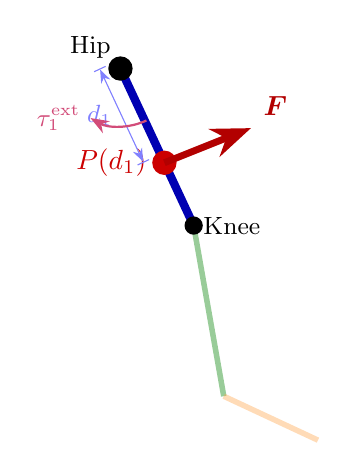
\begin{tikzpicture}[scale=2.2, >=Stealth]
    % Thigh
    \coordinate (hip) at (0,0);
    \coordinate (knee) at ({1.0*sin(25)},{-1.0*cos(25)});
    \draw[blue!70!black, line width=3pt] (hip) -- (knee);

    % Shank
    \coordinate (ankle) at ($(knee) + ({1.0*sin(10)},{-1.0*cos(10)})$);
    \draw[green!50!black, line width=2pt, opacity=0.4] (knee) -- (ankle);

    % Foot
    \coordinate (toe) at ($(ankle) + ({0.6*sin(65)},{-0.6*cos(65)})$);
    \draw[orange!70, line width=2pt, opacity=0.4] (ankle) -- (toe);

    % Force application point on thigh
    \coordinate (Pf) at ($(hip)!0.6!(knee)$);
    \fill[red!80!black] (Pf) circle (2pt);
    \node[left=3pt, red!80!black] at (Pf) {$P(d_1)$};

    % Force arrow
    \draw[->, red!70!black, line width=2.5pt] (Pf) -- ($(Pf) + (0.5, 0.2)$)
        node[above right]{$\vc{F}$};

    % Distance label
    \draw[|<->|, blue!50] ($(hip) + (-0.12,0)$) -- ($(Pf) + (-0.12,0)$)
        node[midway, left]{\small $d_1$};

    % Joints
    \fill[black] (hip) circle (2pt) node[above left]{\small Hip};
    \fill[black] (knee) circle (1.5pt) node[right]{\small Knee};

    % Torque arc at hip
    \draw[->, purple!70, thick] (0.15, -0.3) arc[start angle=295, end angle=240, radius=0.35]
        node[left]{\small $\tau_1^{\text{ext}}$};
\end{tikzpicture}
\caption{External force on the thigh at distance $d_1$ from the hip.
Only the hip joint torque $\tau_1$ is generated.}
\label{fig:force_on_thigh}
\end{figure}

A force applied at distance $d_1$ from the hip along the thigh:
\begin{equation}
    \vc{p}(d_1) = \begin{bmatrix} d_1 \sin\theta_1 \\ -d_1 \cos\theta_1 \end{bmatrix}
\end{equation}

\textbf{Point Jacobian:}
\begin{equation}
    \vc{J}_{p} = \begin{bmatrix}
        d_1 \cos\theta_1 & 0 & 0 \\
        d_1 \sin\theta_1 & 0 & 0
    \end{bmatrix}
    \label{eq:J_thigh}
\end{equation}

\begin{resultbox}[Joint Torques from Force on Thigh]
\begin{align}
    \tau_1^{\text{ext}} &= d_1 (F_x \cos\theta_1 + F_y \sin\theta_1)
                        = d_1 \|\vc{F}\| \sin(\alpha - \theta_1 + \tfrac{\pi}{2}) \label{eq:tau1_thigh} \\
    \tau_2^{\text{ext}} &= 0 \label{eq:tau2_thigh} \\
    \tau_3^{\text{ext}} &= 0 \label{eq:tau3_thigh}
\end{align}
where $\alpha = \text{atan2}(F_y, F_x)$ is the force direction.

\textbf{Key insight}: A force on the thigh affects \textit{only the hip joint}.
The knee and ankle are unaffected because the thigh is proximal to both.
\end{resultbox}

\subsubsection*{2D Cross Product (Moment Arm) Interpretation}

The torque about the hip can also be written as a 2D cross product:
\begin{equation}
    \tau_1^{\text{ext}} = \vc{r} \times \vc{F} = r_x F_y - r_y F_x
    = d_1 \sin\theta_1 \cdot F_y - (-d_1 \cos\theta_1) \cdot F_x
\end{equation}
where $\vc{r} = \vc{p} - \vc{p}_{\text{hip}}$. The effective moment arm is
$d_{\perp} = d_1 \sin\phi$, where $\phi$ is the angle between the force
direction and the thigh axis.

\subsection{Case 2: Force Applied on the Shank}

A force at distance $d_2$ from the knee along the shank:
\begin{equation}
    \vc{p}(d_2) = \begin{bmatrix}
        l_1 \sin\theta_1 + d_2 \sin\theta_2 \\
        -l_1 \cos\theta_1 - d_2 \cos\theta_2
    \end{bmatrix}
\end{equation}

\textbf{Point Jacobian:}
\begin{equation}
    \vc{J}_{p} = \begin{bmatrix}
        l_1 \cos\theta_1 & d_2 \cos\theta_2 & 0 \\
        l_1 \sin\theta_1 & d_2 \sin\theta_2 & 0
    \end{bmatrix}
    \label{eq:J_shank}
\end{equation}

\begin{resultbox}[Joint Torques from Force on Shank]
\begin{align}
    \tau_1^{\text{ext}} &= l_1 (F_x \cos\theta_1 + F_y \sin\theta_1)
    \label{eq:tau1_shank} \\
    \tau_2^{\text{ext}} &= d_2 (F_x \cos\theta_2 + F_y \sin\theta_2)
    \label{eq:tau2_shank} \\
    \tau_3^{\text{ext}} &= 0 \label{eq:tau3_shank}
\end{align}

\textbf{Key insight}: A force on the shank creates torques at \textit{both
hip and knee}, but \textit{not the ankle}. The hip torque depends on the
\textit{full thigh length} $l_1$ (not the point of application), because
the entire thigh acts as a rigid lever arm.
\end{resultbox}

\subsubsection*{Moment Arm Analysis}

\begin{align}
    \text{Moment arm about hip:}\quad
    & d_{\perp,\text{hip}} = \bigl\|\vc{p}(d_2) - \vc{p}_{\text{hip}}\bigr\| \sin\phi_{\text{hip}} \nonumber \\
    \text{Moment arm about knee:}\quad
    & d_{\perp,\text{knee}} = \bigl\|\vc{p}(d_2) - \vc{p}_{\text{knee}}\bigr\| \sin\phi_{\text{knee}}
    = d_2 \sin\phi_{\text{knee}}
\end{align}
where $\phi$ is the angle between the force and the position vector from the joint.

\subsubsection*{Torque Ratio}

The ratio of hip torque to knee torque:
\begin{equation}
    \frac{\tau_1^{\text{ext}}}{\tau_2^{\text{ext}}}
    = \frac{l_1 (F_x \cos\theta_1 + F_y \sin\theta_1)}
           {d_2 (F_x \cos\theta_2 + F_y \sin\theta_2)}
    \label{eq:torque_ratio_shank}
\end{equation}

When $\theta_1 \approx \theta_2$ (thigh and shank nearly aligned):
$\tau_1/\tau_2 \approx l_1/d_2$, which is purely geometric.

\subsection{Case 3: Force Applied on the Foot}

A force at distance $d_3$ from the ankle along the foot:
\begin{equation}
    \vc{p}(d_3) = \begin{bmatrix}
        l_1 \sin\theta_1 + l_2 \sin\theta_2 + d_3 \sin\theta_3 \\
        -l_1 \cos\theta_1 - l_2 \cos\theta_2 - d_3 \cos\theta_3
    \end{bmatrix}
\end{equation}

\textbf{Point Jacobian:}
\begin{equation}
    \vc{J}_{p} = \begin{bmatrix}
        l_1 \cos\theta_1 & l_2 \cos\theta_2 & d_3 \cos\theta_3 \\
        l_1 \sin\theta_1 & l_2 \sin\theta_2 & d_3 \sin\theta_3
    \end{bmatrix}
    \label{eq:J_foot}
\end{equation}

\begin{resultbox}[Joint Torques from Force on Foot --- All 3 Joints Affected]
\begin{align}
    \tau_1^{\text{ext}} &= l_1 (F_x \cos\theta_1 + F_y \sin\theta_1) \label{eq:tau1_foot} \\
    \tau_2^{\text{ext}} &= l_2 (F_x \cos\theta_2 + F_y \sin\theta_2) \label{eq:tau2_foot} \\
    \tau_3^{\text{ext}} &= d_3 (F_x \cos\theta_3 + F_y \sin\theta_3) \label{eq:tau3_foot}
\end{align}

\textbf{Key insight}: A force on the foot creates torques at
\textit{all three joints}. The hip and knee torques depend on the
\textit{full segment lengths} $l_1, l_2$ respectively, independent of where
on the foot the force is applied. Only the ankle torque depends on the
application point $d_3$.
\end{resultbox}

\subsubsection*{Special Case: Ground Reaction Force (GRF)}

During stance, the GRF acts at the foot-ground contact point (approximately at $d_3 \approx l_3/2$
for mid-foot contact). A typical GRF of $\vc{F}_{\text{GRF}} = [F_x^{\text{GRF}}, F_y^{\text{GRF}}]^T$
where $F_y^{\text{GRF}} \approx M_{\text{body}} g$ produces:
\begin{align}
    \tau_1^{\text{GRF}} &= l_1 (F_x^{\text{GRF}} \cos\theta_1 + F_y^{\text{GRF}} \sin\theta_1) \\
    \tau_2^{\text{GRF}} &= l_2 (F_x^{\text{GRF}} \cos\theta_2 + F_y^{\text{GRF}} \sin\theta_2) \\
    \tau_3^{\text{GRF}} &= d_3 (F_x^{\text{GRF}} \cos\theta_3 + F_y^{\text{GRF}} \sin\theta_3)
\end{align}

\subsection{General Case: Force at Arbitrary Point with Offset}

In practice (e.g., H-Walker cable), forces may be applied at a point
that is \textit{offset} from the link axis. For a force applied at:
\begin{equation}
    \vc{p}_{\text{offset}} = \vc{p}_{\text{joint}} + d_{\parallel}
    \begin{bmatrix} \sin\theta_k \\ -\cos\theta_k \end{bmatrix}
    + d_{\perp}
    \begin{bmatrix} -\cos\theta_k \\ -\sin\theta_k \end{bmatrix}
    \label{eq:offset_point}
\end{equation}
where $d_{\parallel}$ is the distance along the link and $d_{\perp}$ is the
perpendicular offset (e.g., posterior side), the Jacobian column for joint $k$
gains an additional term from the offset:
\begin{equation}
    \pder{\vc{p}_{\text{offset}}}{\theta_k} =
    \begin{bmatrix}
        d_{\parallel}\cos\theta_k + d_{\perp}\sin\theta_k \\
        d_{\parallel}\sin\theta_k - d_{\perp}\cos\theta_k
    \end{bmatrix}
    \label{eq:J_offset_column}
\end{equation}

This is exactly the formulation used for the H-Walker cable attachment
in \cref{sec:cable_mapping}.

\subsection{Summary: Force Application Rules}

\begin{table}[H]
\centering
\caption{Which joints are affected by force application at each link.}
\label{tab:force_rules}
\begin{tabular}{@{}lccc l@{}}
\toprule
\textbf{Force on} & $\tau_1$ (Hip) & $\tau_2$ (Knee) & $\tau_3$ (Ankle) & \textbf{Jacobian columns} \\
\midrule
Thigh (at $d_1$) & $\checkmark$ & $\times$ & $\times$ & $[d_1, 0, 0]$ \\
Shank (at $d_2$) & $\checkmark$ & $\checkmark$ & $\times$ & $[l_1, d_2, 0]$ \\
Foot  (at $d_3$) & $\checkmark$ & $\checkmark$ & $\checkmark$ & $[l_1, l_2, d_3]$ \\
\bottomrule
\end{tabular}
\end{table}

\begin{keybox}[Fundamental Rule]
A force applied at any point on link $k$ produces torques at joint $k$
and \textbf{all joints proximal to it} (joints 1 through $k$).
Joints \textbf{distal} to the force application point (joints $k+1$ through 3)
are \textbf{unaffected}.

\smallskip
The torque at a proximal joint $j < k$ depends on the \textbf{full length}
$l_j$ of the intervening link, not on where the force is applied.
Only the torque at joint $k$ itself depends on the distance $d_k$ from
the proximal joint to the force application point.
\end{keybox}

\subsection{Kinematic Response to Applied Force}

Given an applied force $\vc{F}$ at point $\vc{p}$, the resulting
\textbf{joint accelerations} (assuming no muscle torque) are:
\begin{equation}
\boxed{
    \ddt{\vc{q}} = \mat{M}^{-1}(\vc{q})\bigl[\vc{J}_p^T \vc{F} - \vc{C}\dt{\vc{q}} - \vc{G}\bigr]
}
\label{eq:accel_from_force}
\end{equation}

The \textbf{acceleration of the force application point} itself is:
\begin{equation}
    \ddt{\vc{p}} = \vc{J}_p \ddt{\vc{q}} + \dt{\vc{J}}_p \dt{\vc{q}}
    \label{eq:point_accel}
\end{equation}

\subsubsection*{Operational Space Dynamics}

Projecting the dynamics into Cartesian space at the force application point:
\begin{equation}
    \vc{\Lambda}_p(\vc{q}) \, \ddt{\vc{p}} + \vc{\mu}_p(\vc{q},\dt{\vc{q}}) + \vc{p}_p(\vc{q})
    = \vc{F}
    \label{eq:operational_space}
\end{equation}
where $\vc{\Lambda}_p = (\vc{J}_p \mat{M}^{-1} \vc{J}_p^T)^{-1}$ is the
\textbf{operational space inertia} (the apparent mass felt at point $\vc{p}$).

This tells us: if you push on the shank with force $\vc{F}$, the acceleration
you feel is governed by $\vc{\Lambda}_p$, which depends on the \textit{entire}
chain's inertia projected through the Jacobian.

\subsubsection*{Numerical Example}

For a 70 kg, 1.75 m subject in mid-swing ($\theta_1 = 20°$, $\theta_2 = 45°$,
$\theta_3 = 30°$), applying $\vc{F} = [0, -50]^T$ N (50 N downward) at the
mid-shank ($d_2 = l_2/2 = 0.215$ m):
\begin{align*}
    \tau_1^{\text{ext}} &= 0.4287 \times (0 \cdot \cos 20° + (-50) \cdot \sin 20°)
                        = 0.4287 \times (-17.10) = -7.33 \;\text{N\,m} \\
    \tau_2^{\text{ext}} &= 0.2153 \times (0 \cdot \cos 45° + (-50) \cdot \sin 45°)
                        = 0.2153 \times (-35.36) = -7.61 \;\text{N\,m} \\
    \tau_3^{\text{ext}} &= 0
\end{align*}

The 50 N force at mid-shank creates approximately equal torques at hip ($-7.33$ Nm)
and knee ($-7.61$ Nm), both tending toward extension.

\subsection{Multiple Simultaneous Forces}

When multiple forces are applied simultaneously (e.g., cable force + GRF +
assistive device), the generalized forces simply \textbf{superpose}:
\begin{equation}
    \vc{\tau}^{\text{ext}}_{\text{total}} = \sum_{k} \vc{J}_{p_k}^T \vc{F}_k
    \label{eq:superposition}
\end{equation}

For the H-Walker during stance phase:
\begin{equation}
    \mat{M}\ddt{\vc{q}} + \vc{C}\dt{\vc{q}} + \vc{G}
    = \vc{\tau}_{\text{muscle}}
    + \underbrace{\vc{J}_{\text{cable}}^T \vc{F}_{\text{cable}}}_{\text{H-Walker assist}}
    + \underbrace{\vc{J}_{\text{GRF}}^T \vc{F}_{\text{GRF}}}_{\text{ground reaction}}
    \label{eq:eom_full_forces}
\end{equation}

% ======================================================================
% SECTION 13: CABLE FORCE MAPPING
% ======================================================================
\section{H-Walker Cable Force Mapping}
\label{sec:cable_mapping}

\subsection{Cable Geometry}

The H-Walker uses cables from motor spools to assist knee flexion during
the swing phase. The cable attaches on the \textbf{posterior side of the shank},
below the knee, and routes forward to a \textbf{pulley on the walker frame}
in front of the hip.

\begin{figure}[H]
\centering
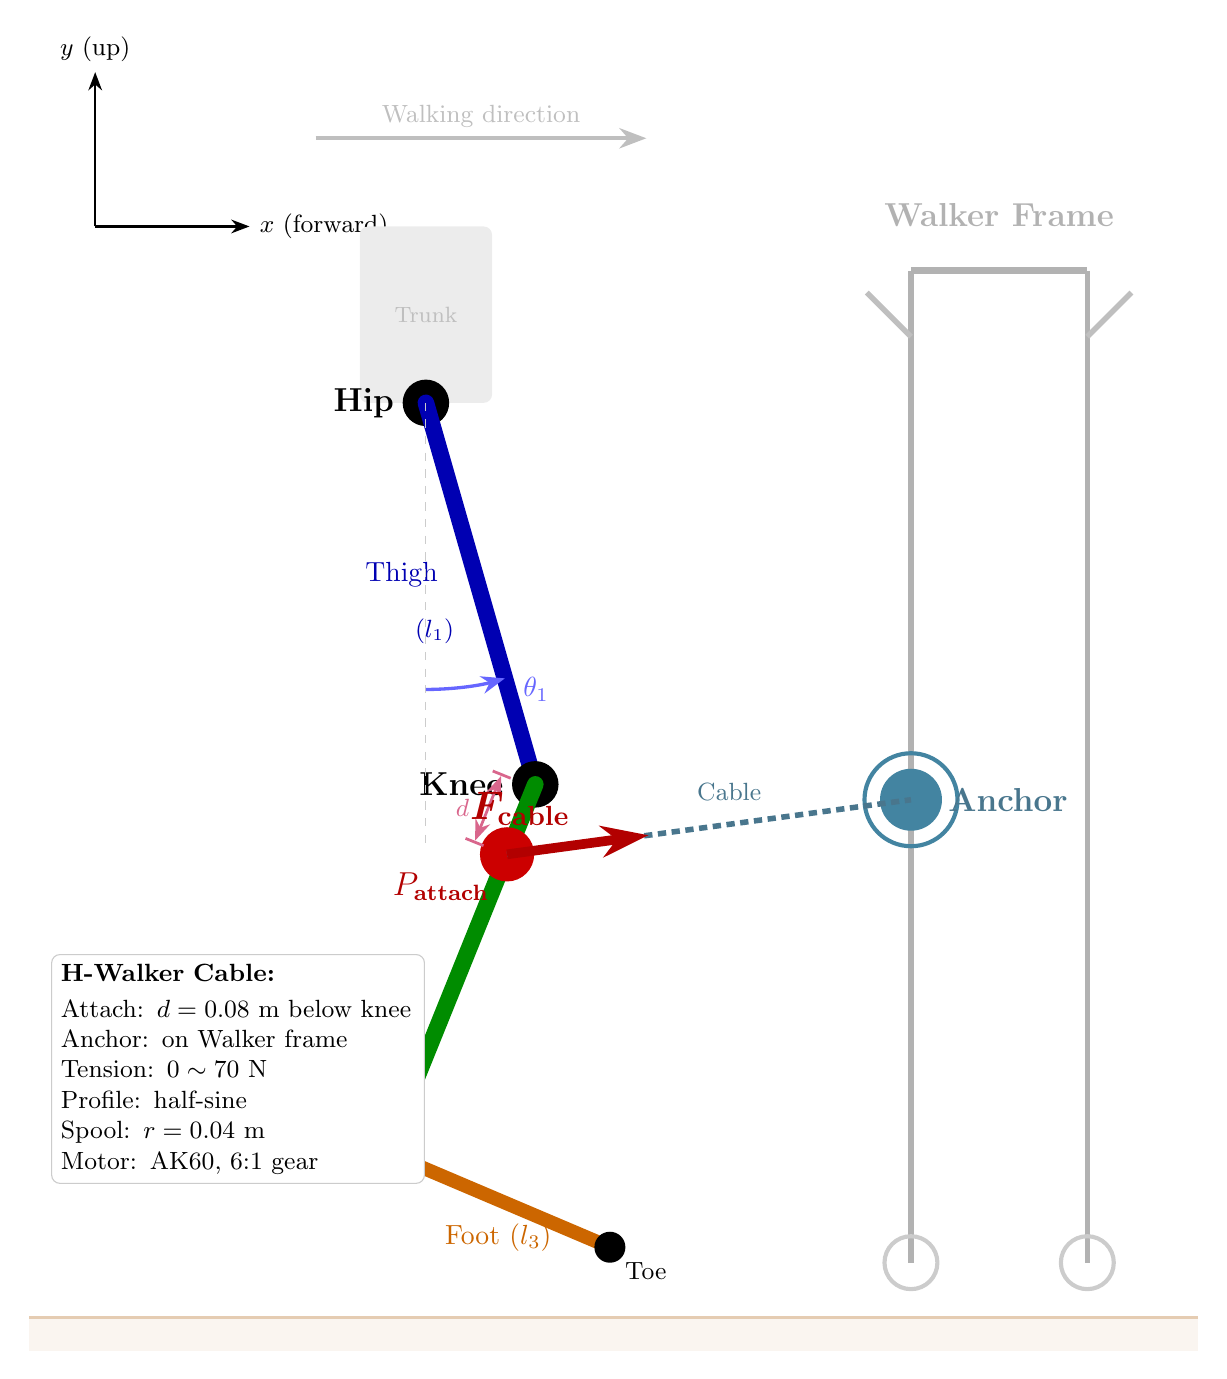
\begin{tikzpicture}[scale=2.8, >=Stealth]
    % ── Ground ──
    \fill[brown!8] (-1.8, -4.3) rectangle (3.5, -4.15);
    \draw[brown!40, line width=1pt] (-1.8, -4.15) -- (3.5, -4.15);

    % ── Coordinate axes (top-left, out of the way) ──
    \draw[->, thick, black] (-1.5, 0.8) -- (-0.8, 0.8) node[right]{\small $x$ (forward)};
    \draw[->, thick, black] (-1.5, 0.8) -- (-1.5, 1.5) node[above]{\small $y$ (up)};

    % ── Walking direction ──
    \draw[->, gray!50, line width=1.5pt] (-0.5, 1.2) -- (1.0, 1.2)
        node[midway, above, gray!50, font=\small]{Walking direction};

    % ══════════════════════════════════════════════
    % LEFT SIDE: Person with 3-link leg
    % ══════════════════════════════════════════════

    % ── Trunk (simple rectangle for context) ──
    \fill[gray!15, rounded corners=3pt] (-0.3, 0.0) rectangle (0.3, 0.8);
    \node[gray!50, font=\footnotesize] at (0, 0.4) {Trunk};

    % ── Hip joint ──
    \coordinate (hip) at (0, 0);
    \fill[black] (hip) circle (3pt);
    \node[left=8pt, font=\large\bfseries] at (hip) {Hip};

    % ── Thigh: θ₁ ≈ 16° forward ──
    \coordinate (knee) at ({1.8*sin(16)}, {-1.8*cos(16)});
    \draw[blue!70!black, line width=6pt, line cap=round] (hip) -- (knee);
    \node[blue!70!black, left=10pt, font=\normalsize] at ($(hip)!0.45!(knee)$) {Thigh};
    \node[blue!70!black, left=10pt, font=\small] at ($(hip)!0.6!(knee)$) {($l_1$)};

    % ── Knee joint ──
    \fill[black] (knee) circle (3pt);
    \node[left=8pt, font=\large\bfseries] at (knee) {Knee};

    % ── Shank: θ₂ ≈ -22° (backward, knee is flexed) ──
    \coordinate (ankle) at ($(knee) + ({1.8*sin(-22)}, {-1.8*cos(-22)})$);
    \draw[green!55!black, line width=6pt, line cap=round] (knee) -- (ankle);
    \node[green!55!black, left=10pt, font=\normalsize] at ($(knee)!0.5!(ankle)$) {Shank};
    \node[green!55!black, left=10pt, font=\small] at ($(knee)!0.65!(ankle)$) {($l_2$)};

    % ── Ankle joint ──
    \fill[black] (ankle) circle (2.5pt);
    \node[left=8pt, font=\large\bfseries] at (ankle) {Ankle};

    % ── Foot ──
    \coordinate (toe) at ($(ankle) + ({1.1*sin(67)}, {-1.1*cos(67)})$);
    \draw[orange!80!black, line width=5pt, line cap=round] (ankle) -- (toe);
    \node[orange!80!black, below=5pt, font=\normalsize] at ($(ankle)!0.5!(toe)$) {Foot ($l_3$)};

    % ── Toe ──
    \fill[black] (toe) circle (2pt);
    \node[below right=2pt, font=\small] at (toe) {Toe};

    % ── Vertical reference lines (for angle definition) ──
    \draw[dashed, gray!40, thin] (hip) -- ($(hip)+(0,-2.0)$);

    % ── θ₁ angle arc ──
    \draw[blue!60, line width=1.2pt, -{Stealth[length=3mm]}]
        ($(hip)+(0,-1.3)$) arc[start angle=270, end angle=286, radius=1.3];
    \node[blue!60, font=\normalsize] at ($(hip)+(0.5,-1.3)$) {$\theta_1$};

    % ══════════════════════════════════════════════
    % CABLE: Attach → Anchor
    % ══════════════════════════════════════════════

    % ── P_attach on shank (8cm below knee ≈ 18.6% of shank) ──
    \coordinate (attach) at ($(knee)!0.19!(ankle)$);
    \fill[red!80!black] (attach) circle (3.5pt);
    \node[below left=3pt, red!70!black, font=\large\bfseries] at (attach) {$P_{\text{attach}}$};

    % ── d annotation (knee to attach) ──
    \draw[|<->|, purple!60, line width=1pt]
        ($(knee)+(-0.15, 0.05)$) -- ($(attach)+(-0.15, 0.05)$)
        node[midway, left=3pt, purple!60, font=\small] {$d$};

    % ══════════════════════════════════════════════
    % RIGHT SIDE: Walker frame with Anchor
    % ══════════════════════════════════════════════

    % ── Walker frame ──
    \draw[gray!60, line width=2.5pt] (2.2, 0.6) -- (3.0, 0.6);   % top bar
    \draw[gray!60, line width=2pt] (2.2, 0.6) -- (2.2, -3.9);    % left leg
    \draw[gray!60, line width=2pt] (3.0, 0.6) -- (3.0, -3.9);    % right leg
    % Wheels
    \draw[gray!40, line width=1.5pt] (2.2, -3.9) circle (0.12);
    \draw[gray!40, line width=1.5pt] (3.0, -3.9) circle (0.12);
    % Handle
    \draw[gray!50, line width=2pt] (2.2, 0.3) -- (2.0, 0.5);
    \draw[gray!50, line width=2pt] (3.0, 0.3) -- (3.2, 0.5);
    \node[gray!60, font=\large\bfseries] at (2.6, 0.85) {Walker Frame};

    % ── Anchor point on walker (at roughly knee height) ──
    \coordinate (anchor) at (2.2, -1.8);
    \fill[cyan!60!black] (anchor) circle (4pt);
    \draw[cyan!60!black, line width=1.5pt] (anchor) circle (6pt);
    \node[right=10pt, cyan!50!black, font=\large\bfseries] at (anchor) {Anchor};

    % ══════════════════════════════════════════════
    % CABLE LINE + FORCE ARROW
    % ══════════════════════════════════════════════

    % ── Cable (dashed line from attach to anchor) ──
    \draw[cyan!50!black, line width=2pt, densely dashed] (attach) -- (anchor);
    \node[cyan!50!black, above=5pt, font=\small] at ($(attach)!0.55!(anchor)$) {Cable};

    % ── Force arrow (from attach toward anchor, prominent) ──
    \draw[-{Stealth[length=6mm, width=4mm]}, red!70!black, line width=3.5pt]
        (attach) -- ($(attach)!0.35!(anchor)$);
    \node[red!70!black, above left=3pt, font=\Large\bfseries]
        at ($(attach)!0.20!(anchor)$) {$\vc{F}_{\text{cable}}$};

    % ══════════════════════════════════════════════
    % INFO BOX (bottom-left, no overlap)
    % ══════════════════════════════════════════════
    \node[draw=gray!40, fill=white, rounded corners=3pt, font=\small,
          text width=4.5cm, align=left, anchor=north west] at (-1.7, -2.5) {
        \textbf{H-Walker Cable:}\\[2pt]
        Attach: $d = 0.08$ m below knee\\
        Anchor: on Walker frame\\
        Tension: $0 \sim 70$ N\\
        Profile: half-sine\\
        Spool: $r = 0.04$ m\\
        Motor: AK60, 6:1 gear
    };
\end{tikzpicture}
\caption{H-Walker cable routing in the sagittal plane.
\textbf{Left}: 3-link leg model (thigh--shank--foot) with cable attachment
$P_{\text{attach}}$ on the shank ($d$ below knee).
\textbf{Right}: Walker frame in front of the person with Anchor point.
The cable connects $P_{\text{attach}} \to \text{Anchor}$, and the force
$\vc{F}_{\text{cable}}$ pulls the shank forward toward the walker.}
\label{fig:cable_geometry}
\end{figure}

\subsection{Cable Attachment Point}

The attachment point in the world frame:
\begin{equation}
    \vc{p}_{\text{attach}} = \vc{p}_{\text{knee}}
    + d_{\parallel} \begin{bmatrix} \sin\theta_2 \\ -\cos\theta_2 \end{bmatrix}
    + d_{\perp} \begin{bmatrix} -\cos\theta_2 \\ -\sin\theta_2 \end{bmatrix}
    \label{eq:cable_attach}
\end{equation}
where $d_{\parallel}$ is the distance along the shank and $d_{\perp}$ is the
posterior offset.

Expanded:
\begin{equation}
    \vc{p}_{\text{attach}} = \begin{bmatrix}
        l_1 \sin\theta_1 + d_{\parallel}\sin\theta_2 - d_{\perp}\cos\theta_2 \\
        -l_1 \cos\theta_1 - d_{\parallel}\cos\theta_2 - d_{\perp}\sin\theta_2
    \end{bmatrix}
    \label{eq:cable_attach_expanded}
\end{equation}

\subsection{Cable Direction and Force Vector}

The unit direction from attachment to pulley:
\begin{equation}
    \hat{\vc{u}} = \frac{\vc{p}_{\text{pulley}} - \vc{p}_{\text{attach}}}
                        {\|\vc{p}_{\text{pulley}} - \vc{p}_{\text{attach}}\|}
    \label{eq:cable_direction}
\end{equation}

The cable force vector (tension is always positive, cable can only pull):
\begin{equation}
    \vc{F}_{\text{cable}} = T_{\text{cable}} \cdot \hat{\vc{u}}, \quad T_{\text{cable}} \geq 0
    \label{eq:cable_force}
\end{equation}

\subsection{Jacobian Mapping: Cable Force to Joint Torques}

Using the principle of virtual work, the generalized forces from the cable are:
\begin{equation}
    Q_i = \vc{F}_{\text{cable}} \cdot \pder{\vc{p}_{\text{attach}}}{\theta_i}
    \label{eq:virtual_work}
\end{equation}

Define the cable Jacobian:
\begin{equation}
    \vc{J}_{\text{cable}} = \pder{\vc{p}_{\text{attach}}}{\vc{q}}
    = \begin{bmatrix}
        l_1 \cos\theta_1 & d_{\parallel}\cos\theta_2 + d_{\perp}\sin\theta_2 & 0 \\
        l_1 \sin\theta_1 & d_{\parallel}\sin\theta_2 - d_{\perp}\cos\theta_2 & 0
    \end{bmatrix}
    \label{eq:cable_jacobian}
\end{equation}

Note that the third column is zero because the cable attaches above the ankle
(i.e., $\vc{p}_{\text{attach}}$ does not depend on $\theta_3$).

\begin{resultbox}[Cable-to-Joint Torque Mapping]
\begin{equation}
    \vc{\tau}_{\text{cable}} = \vc{J}_{\text{cable}}^T \vc{F}_{\text{cable}}
    = T_{\text{cable}} \cdot \vc{J}_{\text{cable}}^T \hat{\vc{u}}
    \label{eq:cable_torque_mapping}
\end{equation}

Expanded:
\begin{align}
    \tau_{\text{cable},1} &= T_{\text{cable}} \bigl(
        l_1 \cos\theta_1 \, \hat{u}_x + l_1 \sin\theta_1 \, \hat{u}_y
    \bigr) \\
    \tau_{\text{cable},2} &= T_{\text{cable}} \bigl(
        (d_{\parallel}\cos\theta_2 + d_{\perp}\sin\theta_2)\hat{u}_x
        + (d_{\parallel}\sin\theta_2 - d_{\perp}\cos\theta_2)\hat{u}_y
    \bigr) \\
    \tau_{\text{cable},3} &= 0
\end{align}
\end{resultbox}

\subsection{Motor--Cable--Force Chain}

The H-Walker uses AK60 motors. The conversion chain is:

\begin{equation}
    \underbrace{I_{\text{motor}}}_{\text{[A]}}
    \xrightarrow{K_t}
    \underbrace{\tau_{\text{motor}}}_{\text{[Nm]}}
    \xrightarrow{N_{\text{gear}} \cdot \eta}
    \underbrace{\tau_{\text{spool}}}_{\text{[Nm]}}
    \xrightarrow{1/r_{\text{spool}}}
    \underbrace{F_{\text{cable}}}_{\text{[N]}}
\end{equation}

\begin{equation}
\boxed{
    F_{\text{cable}} = \frac{I_{\text{motor}} \cdot K_t \cdot N_{\text{gear}} \cdot \eta}{r_{\text{spool}}}
}
\label{eq:motor_to_force}
\end{equation}

With H-Walker parameters:
\begin{equation}
    F_{\text{cable}} = \frac{I \times 0.078 \times 6.0 \times 0.869}{0.04}
                     = I \times 10.17 \;\text{[N/A]}
\end{equation}


% ======================================================================
% SECTION 13: NORMAL GAIT REFERENCE
% ======================================================================
\section{Normal Gait Reference Trajectories}

\subsection{Fourier Series Representation}

Normal gait joint angles are periodic and well-represented by a Fourier series
(Winter, 2009):
\begin{equation}
    \theta(t) = a_0 + \sum_{n=1}^{N} \left[
        a_n \cos\left(\frac{2\pi n t}{T}\right) + b_n \sin\left(\frac{2\pi n t}{T}\right)
    \right]
    \label{eq:fourier}
\end{equation}
where $T$ is the gait cycle duration and $N = 6$ harmonics provide excellent accuracy.

\subsection{Gait Cycle Phases}

\begin{table}[H]
\centering
\caption{Normal gait cycle phases (heel strike = 0\%).}
\label{tab:gait_phases}
\begin{tabular}{@{}clll@{}}
\toprule
\textbf{GCP [\%]} & \textbf{Phase} & \textbf{Sub-phase} & \textbf{Key Event} \\
\midrule
0     & Stance & Loading Response & Heel Strike \\
0--10 & Stance & Loading Response & Weight acceptance \\
10--30 & Stance & Mid Stance & Single limb support \\
30--50 & Stance & Terminal Stance & Heel rise \\
50--60 & Stance & Pre-Swing & Toe Off ($\approx 60\%$) \\
\midrule
60--73 & Swing & Initial Swing & Foot clearance \\
73--87 & Swing & Mid Swing & Limb advancement \\
87--100 & Swing & Terminal Swing & Deceleration \\
\bottomrule
\end{tabular}
\end{table}

\subsection{Normal Joint Angle Profiles}

From Winter (2009), natural cadence ($\approx 108$ steps/min):

\begin{table}[H]
\centering
\caption{Key joint angle values during normal gait (degrees).}
\label{tab:normal_angles}
\begin{tabular}{@{}lccc@{}}
\toprule
\textbf{Event} & \textbf{Hip Flex/Ext} & \textbf{Knee Flex} & \textbf{Ankle Dorsi/Plantar} \\
\midrule
Heel Strike (0\%)    & $+25^\circ$ & $\approx 5^\circ$ & $\approx 0^\circ$ \\
Loading Response (8\%) & $+20^\circ$ & $\approx 15^\circ$ & $-5^\circ$ \\
Mid Stance (30\%)     & $0^\circ$   & $\approx 5^\circ$  & $+10^\circ$ \\
Terminal Stance (50\%) & $-10^\circ$ & $\approx 5^\circ$  & $+15^\circ$ \\
Toe Off (60\%)         & $-5^\circ$  & $\approx 40^\circ$ & $-20^\circ$ \\
Mid Swing (73\%)       & $+15^\circ$ & $\approx 65^\circ$ & $+5^\circ$ \\
Terminal Swing (95\%)  & $+30^\circ$ & $\approx 5^\circ$  & $\approx 0^\circ$ \\
\bottomrule
\end{tabular}
\end{table}

\subsection{Angular Velocity (Analytical Derivative)}

The derivative of the Fourier series gives the angular velocity:
\begin{equation}
    \dt{\theta}(t) = \sum_{n=1}^{N} \frac{2\pi n}{T} \left[
        -a_n \sin\left(\frac{2\pi n t}{T}\right) + b_n \cos\left(\frac{2\pi n t}{T}\right)
    \right]
    \label{eq:fourier_velocity}
\end{equation}

This analytical derivative avoids numerical differentiation noise, which is
critical for accurate inverse dynamics computation.

% ======================================================================
% SECTION 14: ANTHROPOMETRIC PARAMETERS
% ======================================================================
\section{Anthropometric Parameters}

\subsection{Winter (2009) Body Segment Parameter Data}

Segment properties are expressed as ratios of total body mass ($M$) and height ($H$):

\begin{table}[H]
\centering
\caption{Body segment parameters from Winter (2009) and Dempster (1955).}
\label{tab:bsp}
\begin{tabular}{@{}lcccc@{}}
\toprule
\textbf{Segment} & \textbf{Mass/M} & \textbf{Length/H} & \textbf{CoM/Length} & \textbf{$\rho$/Length} \\
\midrule
Thigh  & 0.100  & 0.245 & 0.433 & 0.323 \\
Shank  & 0.0465 & 0.246 & 0.433 & 0.302 \\
Foot   & 0.0145 & 0.152 & 0.500 & 0.475 \\
\bottomrule
\end{tabular}
\end{table}

where $\rho/\text{Length}$ is the radius of gyration about CoM as a fraction of segment length.
The moment of inertia is:
\begin{equation}
    I_i = m_i \cdot (\rho_i \cdot l_i)^2 = m_i \cdot \left(\frac{\rho_i}{l_i} \cdot l_i\right)^2
    \label{eq:inertia_calc}
\end{equation}

\subsection{Numerical Values (70 kg, 1.75 m Adult)}

\begin{table}[H]
\centering
\caption{Computed segment parameters for a 70 kg, 1.75 m subject.}
\label{tab:numerical_params}
\begin{tabular}{@{}lccccc@{}}
\toprule
\textbf{Segment} & $m_i$ [kg] & $l_i$ [m] & $l_{c_i}$ [m] & $I_i$ [kg$\cdot$m$^2$] & $\rho_i$ [m] \\
\midrule
Thigh ($i=1$) & 7.000 & 0.4288 & 0.1857 & 0.1342 & 0.1385 \\
Shank ($i=2$) & 3.255 & 0.4305 & 0.1864 & 0.0550 & 0.1300 \\
Foot  ($i=3$) & 1.015 & 0.2660 & 0.1330 & 0.0162 & 0.1264 \\
\bottomrule
\end{tabular}
\end{table}

\subsection{Computed Model Coefficients}

Substituting the numerical values into the model equations:

\begin{table}[H]
\centering
\caption{Numerical coefficients in the equations of motion.}
\label{tab:coefficients}
\begin{tabular}{@{}lrl@{}}
\toprule
\textbf{Coefficient} & \textbf{Value} & \textbf{Expression} \\
\midrule
\multicolumn{3}{l}{\textit{Mass matrix diagonal (constants):}} \\
$M_{11}^*$ & 1.160 kg$\cdot$m$^2$ & $m_1 l_{c_1}^2 + (m_2+m_3)l_1^2 + I_1$ \\
$M_{22}^*$ & 0.356 kg$\cdot$m$^2$ & $m_2 l_{c_2}^2 + m_3 l_2^2 + I_2$ \\
$M_{33}^*$ & 0.034 kg$\cdot$m$^2$ & $m_3 l_{c_3}^2 + I_3$ \\
\midrule
\multicolumn{3}{l}{\textit{Coupling coefficients:}} \\
$\alpha_{12}$ & 0.448 kg$\cdot$m$^2$ & $(m_2 l_{c_2} + m_3 l_2)l_1$ \\
$\alpha_{13}$ & 0.058 kg$\cdot$m$^2$ & $m_3 l_{c_3} l_1$ \\
$\alpha_{23}$ & 0.058 kg$\cdot$m$^2$ & $m_3 l_{c_3} l_2$ \\
\midrule
\multicolumn{3}{l}{\textit{Gravity coefficients:}} \\
$\gamma_1$ & 30.71 N$\cdot$m & $(m_1 l_{c_1} + m_2 l_1 + m_3 l_1)g$ \\
$\gamma_2$ & 10.24 N$\cdot$m & $(m_2 l_{c_2} + m_3 l_2)g$ \\
$\gamma_3$ & 1.32 N$\cdot$m & $m_3 l_{c_3} g$ \\
\bottomrule
\end{tabular}
\end{table}

\subsection{Equations with Numerical Coefficients}

For the 70 kg, 1.75 m subject:

\begin{resultbox}[EOM with Numerical Values]
\begin{align}
    \tau_1 &= 1.160\,\ddt{\theta}_1 + 0.448\cos(\theta_1-\theta_2)\,\ddt{\theta}_2
            + 0.058\cos(\theta_1-\theta_3)\,\ddt{\theta}_3 \nonumber \\
           &\quad - 0.448\sin(\theta_1-\theta_2)\,\dt{\theta}_2^2
            - 0.058\sin(\theta_1-\theta_3)\,\dt{\theta}_3^2
            + 30.71\sin\theta_1 \\[6pt]
    \tau_2 &= 0.448\cos(\theta_1-\theta_2)\,\ddt{\theta}_1 + 0.356\,\ddt{\theta}_2
            + 0.058\cos(\theta_2-\theta_3)\,\ddt{\theta}_3 \nonumber \\
           &\quad + 0.448\sin(\theta_1-\theta_2)\,\dt{\theta}_1^2
            - 0.058\sin(\theta_2-\theta_3)\,\dt{\theta}_3^2
            + 10.24\sin\theta_2 \\[6pt]
    \tau_3 &= 0.058\cos(\theta_1-\theta_3)\,\ddt{\theta}_1 + 0.058\cos(\theta_2-\theta_3)\,\ddt{\theta}_2
            + 0.034\,\ddt{\theta}_3 \nonumber \\
           &\quad + 0.058\sin(\theta_1-\theta_3)\,\dt{\theta}_1^2
            + 0.058\sin(\theta_2-\theta_3)\,\dt{\theta}_2^2
            + 1.32\sin\theta_3
\end{align}
\end{resultbox}

% ======================================================================
% SECTION 15: LINEARIZATION
% ======================================================================
\section{Linearization for Control Design}

For MPC and linear control, we linearize about a reference trajectory
$(\vc{q}_0, \dt{\vc{q}}_0, \vc{\tau}_0)$:

\begin{equation}
    \mat{M}_0 \, \delta\ddt{\vc{q}} + \vc{C}_0 \, \delta\dt{\vc{q}}
    + \vc{K}_0 \, \delta\vc{q} = \delta\vc{\tau}
    \label{eq:linearized}
\end{equation}

where:
\begin{align}
    \mat{M}_0 &= \mat{M}(\vc{q}_0) \\
    \vc{C}_0  &= \vc{C}(\vc{q}_0, \dt{\vc{q}}_0) \\
    \vc{K}_0  &= \pder{(\vc{C}\dt{\vc{q}} + \vc{G})}{\vc{q}}\bigg|_{\vc{q}_0, \dt{\vc{q}}_0}
\end{align}

The stiffness matrix $\vc{K}_0$ includes both the gravitational stiffness
($\partial G_i / \partial q_j$) and the velocity-dependent stiffness from
the Coriolis terms.

For small perturbations about the hanging equilibrium ($\vc{q}_0 = \vc{0}$,
$\dt{\vc{q}}_0 = \vc{0}$):
\begin{equation}
    K_{ij} = \pder{G_i}{\theta_j}\bigg|_{\vc{q}=\vc{0}} = \gamma_i \, \delta_{ij}
\end{equation}
which is diagonal --- the linearized system decouples when hanging straight down.

% ======================================================================
% SECTION 16: MODEL-BASED CONTROL APPLICATION
% ======================================================================
\section{Model-Based Control Application for H-Walker}
\label{sec:control_application}

This section connects the biomechanical model to the actual H-Walker
control problem: \textit{given a fixed cable attachment point, how does
the cable force affect joint torques, angular accelerations, and gait
parameters (stride length, foot clearance) at each instant?}

\subsection{Instantaneous Effect of Cable Force on Gait}

At each time instant during gait (characterized by GCP\%), the cable
force $T_{\text{cable}}$ produces specific joint torques that depend on
the \textit{current leg configuration} $\vc{q}(t)$.

\subsubsection*{Step 1: Cable Force $\to$ Joint Torques}

From \cref{sec:cable_mapping}, at configuration $\vc{q}$:
\begin{equation}
    \vc{\tau}_{\text{cable}}(\vc{q}, T) = T \cdot \vc{J}_{\text{cable}}^T(\vc{q}) \, \hat{\vc{u}}(\vc{q})
    \label{eq:cable_tau_instant}
\end{equation}

The key insight: \textbf{the same cable tension $T$ produces different
torques at different gait phases}, because $\vc{q}$ changes throughout
the gait cycle, which changes both the cable direction $\hat{\vc{u}}$
and the moment arms.

\begin{table}[H]
\centering
\caption{Cable force effect across the gait cycle (50 N tension, 70 kg subject).}
\label{tab:cable_gait_phases}
\begin{tabular}{@{}lcrrrr@{}}
\toprule
\textbf{Phase} & \textbf{GCP} & $\theta_1$ & $\theta_2$ & $\tau_{\text{hip}}$ & $\tau_{\text{knee}}$ \\
\midrule
Pre-swing      & 60\%  & $-6°$  & $17°$ & $-4.2$ Nm & $-0.7$ Nm \\
Initial swing  & 65\%  & $3°$   & $29°$ & $-4.2$ Nm & $-0.7$ Nm \\
Mid-swing      & 73\%  & $17°$  & $46°$ & $-1.7$ Nm & $-0.3$ Nm \\
Terminal swing  & 90\%  & $23°$  & $9°$  & $-1.5$ Nm & $-2.0$ Nm \\
\bottomrule
\end{tabular}
\end{table}

Observation: The cable is most effective for knee flexion assistance
during \textbf{initial swing} (60--65\% GCP) and most effective for
knee extension control during \textbf{terminal swing} (85--95\% GCP).

\subsubsection*{Step 2: Joint Torques $\to$ Angular Accelerations}

The cable-induced torques produce angular accelerations via forward dynamics:
\begin{equation}
    \ddt{\vc{q}}_{\text{cable}} = \mat{M}^{-1}(\vc{q}) \, \vc{\tau}_{\text{cable}}
    \label{eq:cable_accel}
\end{equation}

Note: Due to the mass matrix coupling, the cable force on the shank
affects \textit{all three joint accelerations}, not just hip and knee:
\begin{equation}
    \begin{bmatrix} \ddt{\theta}_{1,\text{cable}} \\ \ddt{\theta}_{2,\text{cable}} \\ \ddt{\theta}_{3,\text{cable}} \end{bmatrix}
    = \mat{M}^{-1}
    \begin{bmatrix} \tau_{\text{cable},1} \\ \tau_{\text{cable},2} \\ 0 \end{bmatrix}
    \neq
    \begin{bmatrix} \tau_{\text{cable},1}/M_{11} \\ \tau_{\text{cable},2}/M_{22} \\ 0 \end{bmatrix}
\end{equation}

The right side is \textbf{wrong} --- you cannot divide each torque by its
diagonal mass element because $\mat{M}$ is coupled. The off-diagonal
elements $M_{31}, M_{32}$ transmit the effect to the ankle even though
$\tau_{\text{cable},3} = 0$.

\subsubsection*{Step 3: Angular Accelerations $\to$ Gait Parameter Changes}

\textbf{Stride length change:}
The foot endpoint velocity determines stride length. Using the endpoint Jacobian:
\begin{equation}
    \Delta \dot{\vc{p}}_{\text{toe}} = \vc{J}_{\text{toe}}(\vc{q}) \cdot \Delta\dot{\vc{q}}
    \quad \Rightarrow \quad
    \Delta\text{stride} \approx \int_{\text{swing}} \Delta \dot{x}_{\text{toe}} \, dt
    \label{eq:stride_change}
\end{equation}

\textbf{Foot clearance change:}
The vertical position of the toe during swing determines ground clearance:
\begin{equation}
    \Delta y_{\text{toe}} = \vc{J}_{\text{toe},y}(\vc{q}) \cdot \Delta\vc{q}
    = l_1 \sin\theta_1 \cdot \Delta\theta_1 + l_2 \sin\theta_2 \cdot \Delta\theta_2 + l_3 \sin\theta_3 \cdot \Delta\theta_3
    \label{eq:clearance_change}
\end{equation}

\textbf{Step time change:}
The angular velocity of the thigh determines stride frequency:
\begin{equation}
    \Delta T_{\text{step}} \approx -\frac{\Delta\dot{\theta}_1}{\dot{\theta}_1^2} \cdot \Delta\theta_{\text{stride}}
    \label{eq:step_time_change}
\end{equation}

\subsection{Complete Gait Cycle Analysis}

The full EOM during cable-assisted walking:
\begin{equation}
\boxed{
    \mat{M}(\vc{q})\ddt{\vc{q}} = \underbrace{\vc{\tau}_{\text{muscle}}}_{\text{patient effort}}
    + \underbrace{\vc{J}_{\text{cable}}^T T_{\text{cable}}  \hat{\vc{u}}}_{\text{H-Walker assist}}
    - \vc{C}(\vc{q},\dt{\vc{q}})\dt{\vc{q}} - \vc{G}(\vc{q})
    + \underbrace{\vc{J}_{\text{GRF}}^T \vc{F}_{\text{GRF}}}_{\text{stance only}}
}
\label{eq:full_gait_eom}
\end{equation}

\subsubsection*{Swing Phase (60--100\% GCP): Cable Assistance is Active}

During swing, $\vc{F}_{\text{GRF}} = \vc{0}$:
\begin{equation}
    \mat{M}\ddt{\vc{q}} + \vc{C}\dt{\vc{q}} + \vc{G}
    = \vc{\tau}_{\text{muscle}} + \vc{J}_{\text{cable}}^T T \hat{\vc{u}}
\end{equation}

The cable force \textbf{reduces the muscle torque needed}:
\begin{equation}
    \vc{\tau}_{\text{muscle}} = \underbrace{\mat{M}\ddt{\vc{q}} + \vc{C}\dt{\vc{q}} + \vc{G}}_{\text{required for desired motion}}
    - \underbrace{\vc{J}_{\text{cable}}^T T \hat{\vc{u}}}_{\text{cable provides this}}
    \label{eq:muscle_reduction}
\end{equation}

This is the \textbf{assist-as-needed} principle: the cable provides part
of the required torque, reducing the patient's effort.

\subsubsection*{Stance Phase (0--60\% GCP): Cable Maintains Pretension}

During stance, the cable maintains minimum tension ($T = 5$ N) to avoid slack.

\subsection{Control Strategies Using This Model}

\subsubsection{Strategy 1: Inverse Dynamics Feedforward (ILC)}

Compute the required cable force to track a desired gait trajectory:
\begin{equation}
    T_{\text{cable}}^{*}(t) = \frac{\bigl[\mat{M}\ddt{\vc{q}}_d + \vc{C}\dt{\vc{q}}_d + \vc{G} - \vc{\tau}_{\text{patient}}\bigr]_{\text{knee}}}
    {\bigl[\vc{J}_{\text{cable}}^T \hat{\vc{u}}\bigr]_{\text{knee}}}
    \label{eq:ilc_feedforward}
\end{equation}

Then ILC refines this across gait cycles:
\begin{equation}
    T_{k+1}(t) = Q\bigl[T_k(t) + L \cdot e_k(t)\bigr]
\end{equation}
where $e_k$ is the tracking error in cycle $k$, $L$ is the learning gain,
and $Q$ is a low-pass filter.

\subsubsection{Strategy 2: Impedance Control with Model Compensation}

Shape the apparent dynamics felt by the patient:
\begin{equation}
    T_{\text{cable}} = \frac{1}{[\vc{J}_{\text{cable}}^T \hat{\vc{u}}]_{\text{knee}}} \bigl[
        \underbrace{\vc{G}_2(\vc{q})}_{\text{gravity comp}}
        + \underbrace{K_v (\dot{\theta}_{2,\text{ref}} - \dot{\theta}_2)}_{\text{virtual damping}}
        + \underbrace{K_p (\theta_{2,\text{ref}} - \theta_2)}_{\text{virtual spring}}
    \bigr]
    \label{eq:impedance_control}
\end{equation}

The model provides $\vc{G}(\vc{q})$ for \textbf{gravity compensation}
so the patient feels the leg is ``weightless'', requiring less effort to swing.

\subsubsection{Strategy 3: MPC with Nonlinear Dynamics}

Use the full model as the prediction model in MPC:
\begin{align}
    \min_{T_{\text{cable}}(t)} \quad & \sum_{k=0}^{N} \bigl\|\vc{q}(t_k) - \vc{q}_{\text{ref}}(t_k)\bigr\|_{\vc{Q}}^2
        + \bigl\|T_{\text{cable}}(t_k)\bigr\|_R^2 \\
    \text{s.t.} \quad & \mat{M}\ddt{\vc{q}} + \vc{C}\dt{\vc{q}} + \vc{G} = \vc{J}_{\text{cable}}^T T \hat{\vc{u}} \\
    & 5 \leq T_{\text{cable}} \leq 70 \;\text{N} \\
    & y_{\text{toe}}(\vc{q}) \geq y_{\text{clearance}} \;\text{(foot clearance constraint)}
\end{align}

The model enables: trajectory prediction, constraint enforcement (max force,
foot clearance), and optimal cable force profiling.

\subsection{Sensitivity Analysis: How Force Direction Affects Gait}

For a fixed attachment point, the cable direction $\hat{\vc{u}}$ changes
with configuration. The \textbf{sensitivity} of each joint torque to
cable tension is:
\begin{equation}
    \vc{s}(\vc{q}) \triangleq \frac{\partial \vc{\tau}_{\text{cable}}}{\partial T}
    = \vc{J}_{\text{cable}}^T(\vc{q}) \, \hat{\vc{u}}(\vc{q})
    = \begin{bmatrix} s_1(\vc{q}) \\ s_2(\vc{q}) \\ 0 \end{bmatrix}
    \label{eq:sensitivity}
\end{equation}

This vector answers: ``\textit{if I increase cable tension by 1 N at this
instant, how much additional torque does each joint get?}''

The sensitivity depends on:
\begin{itemize}
    \item \textbf{Cable angle} relative to each link: perpendicular force
          gives maximum moment arm, parallel gives zero.
    \item \textbf{Leg configuration}: as the leg swings, the cable angle
          changes, so the sensitivity changes throughout the gait cycle.
\end{itemize}

\begin{resultbox}[Practical Design Question]
Given the fixed pulley position on the walker frame, at which GCP\% is
the cable most/least effective?

Answer: Compute $\|\vc{s}(\vc{q}(t))\|$ over one gait cycle.
Peak sensitivity = best time to apply force.
Minimum sensitivity = the cable geometry is unfavorable.

If the sensitivity is too low during a critical phase, the
\textbf{pulley position should be redesigned}.
\end{resultbox}

% ======================================================================
% SECTION 17: SUMMARY
% ======================================================================
\section{Summary}

This document presented the complete nonlinear equations of motion for a
three-link planar biomechanical model of the human lower limb. The key
results are:

\begin{enumerate}
    \item \textbf{Mass matrix} (\cref{eq:mass_matrix}): $3 \times 3$ symmetric
          positive definite, with constant diagonal and configuration-dependent
          off-diagonal elements.
    \item \textbf{Coriolis matrix} (\cref{eq:coriolis_matrix}): Derived via
          Christoffel symbols to ensure the passivity property
          ($\dt{\mat{M}} - 2\vc{C}$ skew-symmetric).
    \item \textbf{Gravity vector} (\cref{eq:G1,eq:G2,eq:G3}): Three
          sinusoidal terms representing gravitational torques.
    \item \textbf{Cable force mapping} (\cref{eq:cable_torque_mapping}):
          Jacobian transpose mapping from cable tension to joint torques.
    \item \textbf{Normal gait reference}: Fourier series with 6 harmonics
          for hip, knee, and ankle angles.
\end{enumerate}

The model supports:
\begin{itemize}
    \item Forward dynamics simulation (ODE integration)
    \item Inverse dynamics (feedforward torque computation)
    \item Energy analysis and conservation verification
    \item Cable-force-aware control design for the H-Walker
    \item Linearization for MPC and impedance control
\end{itemize}

% ======================================================================
% BIBLIOGRAPHY
% ======================================================================
\begin{thebibliography}{10}

\bibitem{winter2009}
Winter, D.A. (2009).
\textit{Biomechanics and Motor Control of Human Movement}, 4th ed.
John Wiley \& Sons.

\bibitem{dempster1955}
Dempster, W.T. (1955).
Space requirements of the seated operator.
WADC Technical Report 55-159, Wright-Patterson AFB.

\bibitem{spong2006}
Spong, M.W., Hutchinson, S., \& Vidyasagar, M. (2006).
\textit{Robot Modeling and Control}.
John Wiley \& Sons.

\bibitem{perry2010}
Perry, J. \& Burnfield, J.M. (2010).
\textit{Gait Analysis: Normal and Pathological Function}, 2nd ed.
SLACK Incorporated.

\bibitem{murray1994}
Murray, R.M., Li, Z., \& Sastry, S.S. (1994).
\textit{A Mathematical Introduction to Robotic Manipulation}.
CRC Press.

\bibitem{umberger2010}
Umberger, B.R. (2010).
Stance and swing phase costs in human walking.
\textit{Journal of the Royal Society Interface}, 7(50), 1329--1340.

\bibitem{sciavicco2000}
Sciavicco, L. \& Siciliano, B. (2000).
\textit{Modelling and Control of Robot Manipulators}, 2nd ed.
Springer.

\bibitem{hairer1993}
Hairer, E., N{\o}rsett, S.P., \& Wanner, G. (1993).
\textit{Solving Ordinary Differential Equations I: Nonstiff Problems}.
Springer.

\end{thebibliography}

\end{document}
